\chapter{胸 痛}

胸痛是临床上常见的症状,表现可轻可重,而疼痛严重程度与病情轻重并不完全一致,其临床意义也可大可小,若起源于局部轻微损害,则意义不大;但如由于内脏疾病引起的疼痛则有重要的临床意义,可由此引起突然死亡。

各种刺激因子如缺氧、炎症、肌张力改变、肿瘤浸润、组织坏死以及化学、物理因素都可刺激肋间神经感觉纤维,刺激支配心脏及主动脉的交感神经纤维,刺激支配气管、支气管及食管的迷走神经纤维或膈神经的感觉纤维等,产生痛觉冲动,并传至大脑皮质的痛觉中枢引起胸痛。最常见的胸痛是心脏疾病引起的胸痛;10\%~20\%的胸痛是由于心脏以外的原因,大部分非心源性胸痛源于胸膜或胸壁;因为肺组织和脏层胸膜缺乏痛觉感受器,因此肺实质即使有严重的病变也可以没有胸痛发生。

此外,当某一内脏与体表某一部位同受某些脊神经后根的传入神经支配时,则来自内脏疾病的痛觉冲动到达大脑皮层后,除可产生局部疼痛外,还可出现相应体表区域的疼痛感觉,称为放射痛。例如心绞痛时除出现胸骨后或心前区压榨样疼痛外,还放射到左肩及左臂内侧疼痛。

根据疼痛的起源,可将胸痛区分为五大类,见表\ref{tab10-1}。

\begin{longtable}{c}
 \caption{胸痛疾病的分类}
 \label{tab10-1}
 \endfirsthead
 \caption[]{胸痛疾病的分类}
 \endhead
 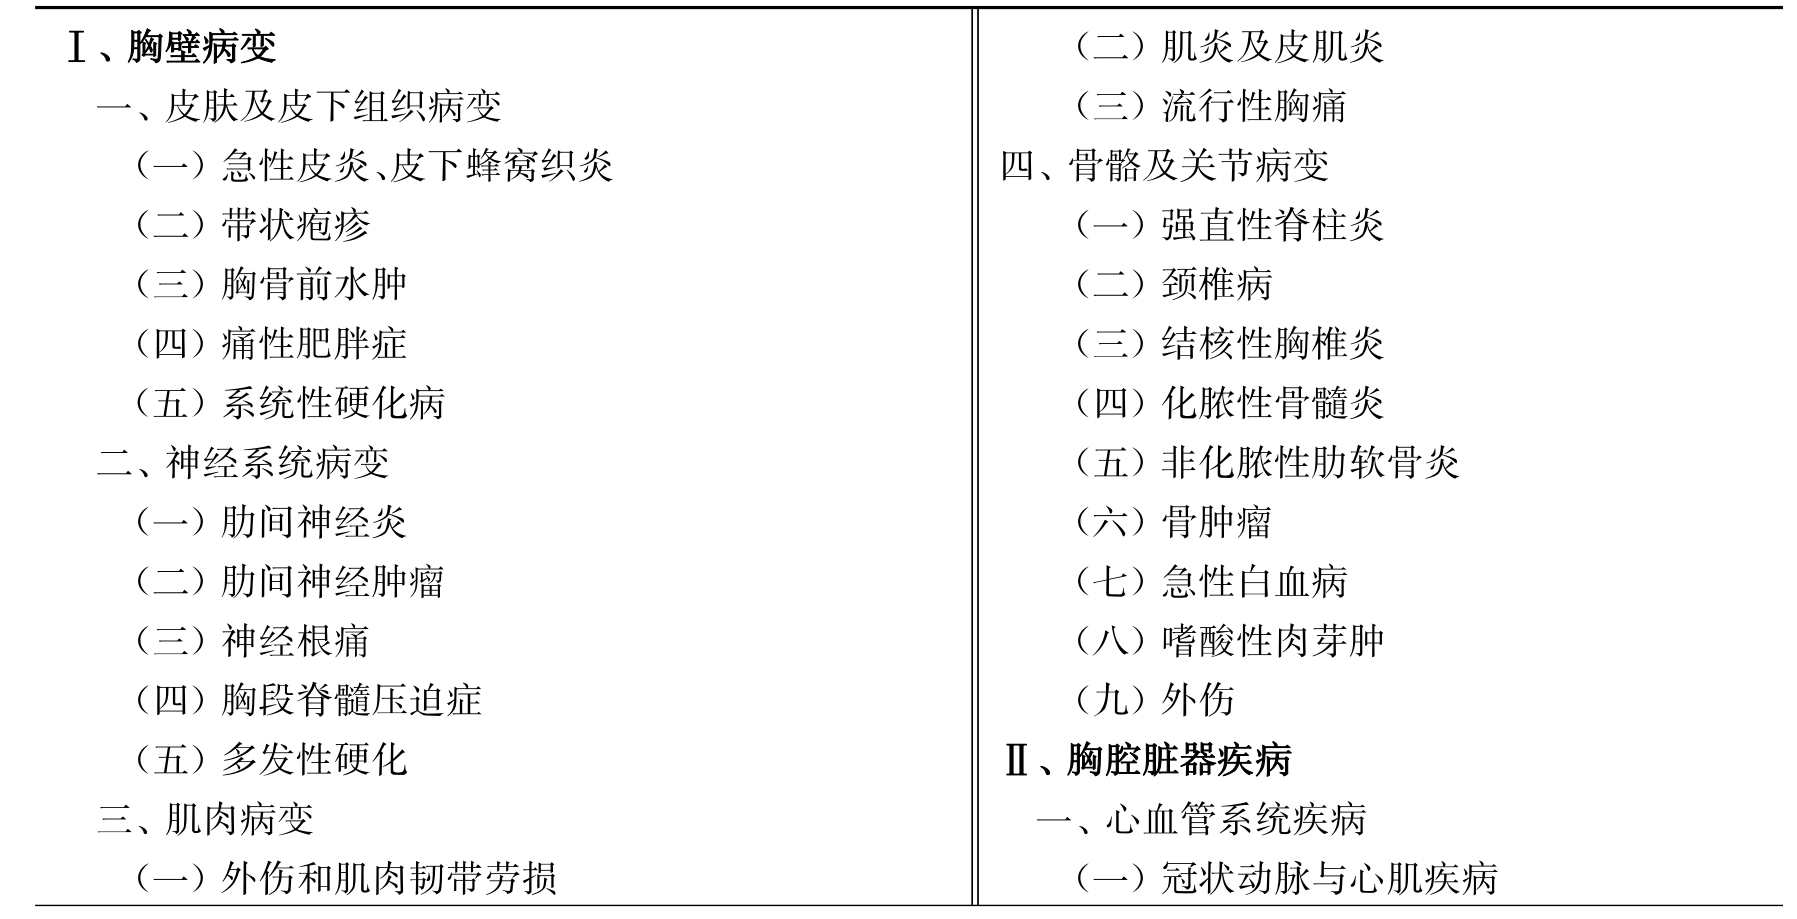
\includegraphics[width=\textwidth,height=\textheight,keepaspectratio]{./images/Image00068.jpg}\\
 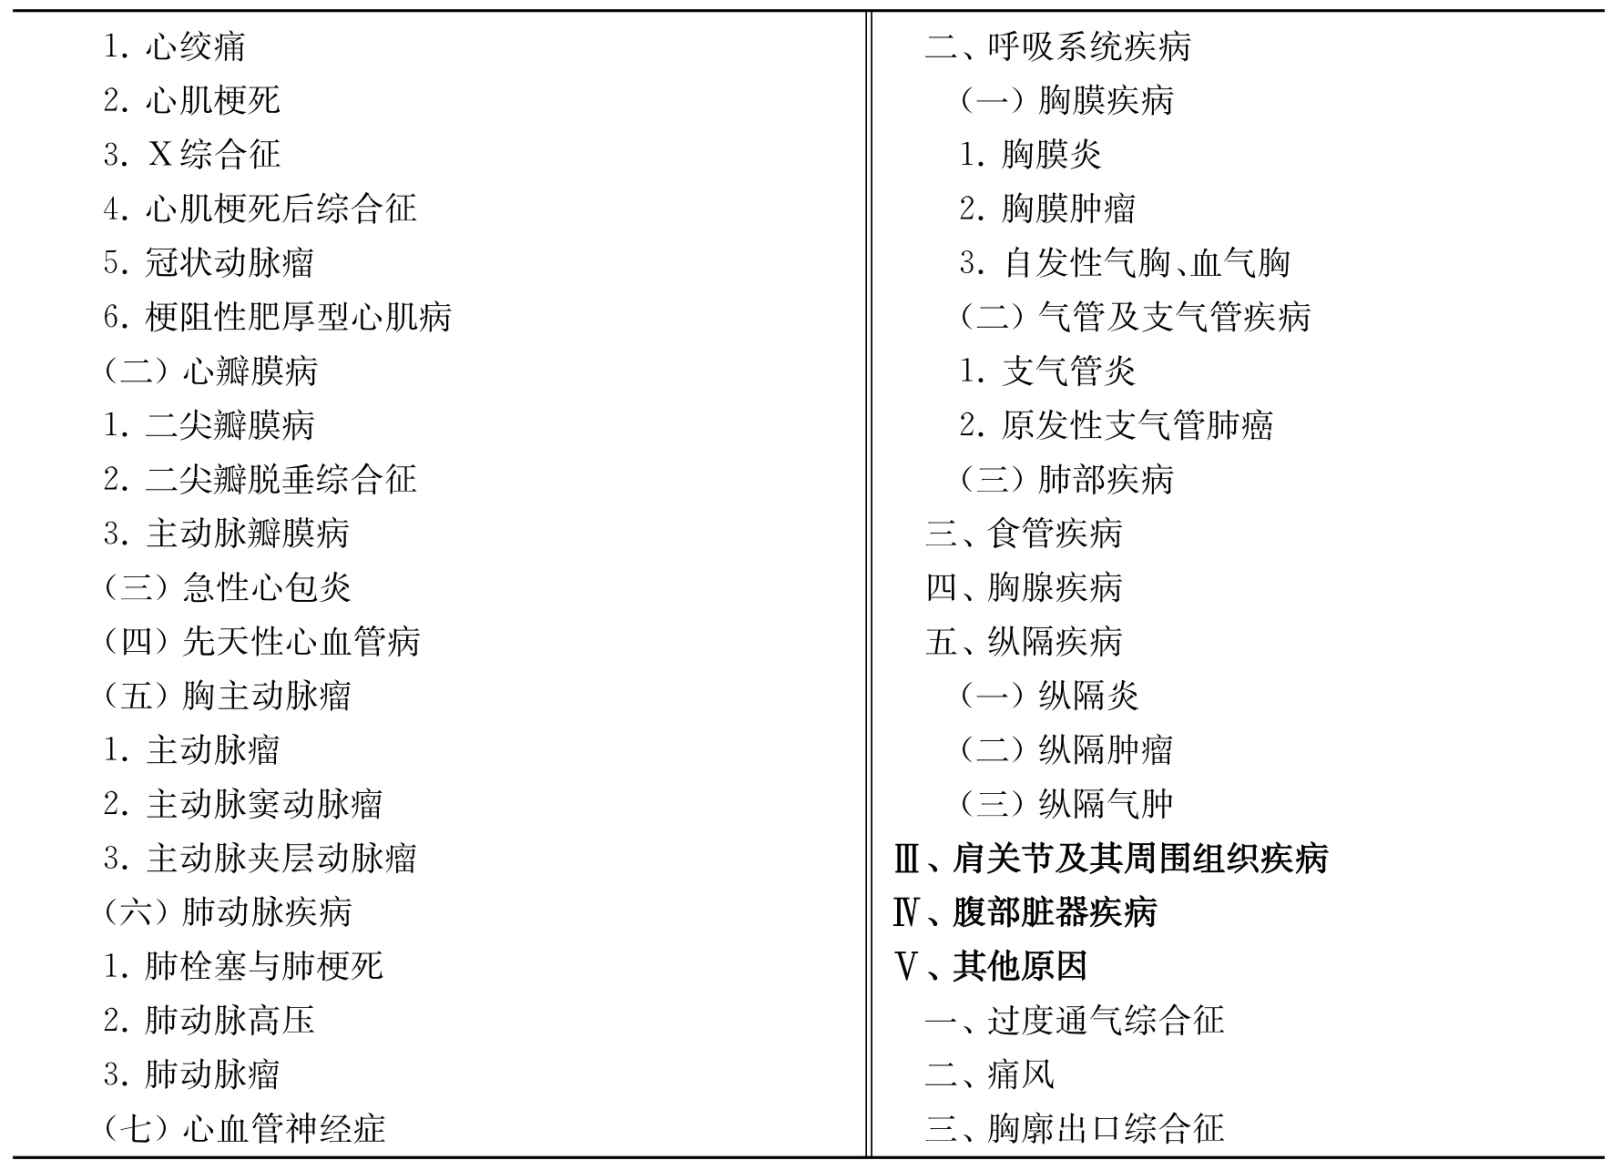
\includegraphics[width=\textwidth,height=\textheight,keepaspectratio]{./images/Image00069.jpg}
 \end{longtable}

下列情况有助于胸痛的诊断与鉴别诊断:

\section{(一)病史}

\subsection{1.发病年龄}

青壮年胸痛,应注意结核性胸膜炎、自发性气胸、心肌炎、心肌病、风湿性心瓣膜病,在40岁以上还应注意心绞痛、心肌梗死与肺癌。

\subsection{2.疼痛部位}

很多疾病引起的胸痛常有一定的部位。如胸壁疾病所致的胸痛常固定于病变部位,且局部多有明显压痛;带状疱疹是成簇水泡沿一侧肋间神经分布并伴剧痛,疱疹不越过体表中线。非化脓性肋骨软骨炎多侵犯第一、二肋软骨,对称或非对称性,呈单个或多个肿胀隆起,局部皮色正常,有压痛,咳嗽、深呼吸或上肢大幅度活动时疼痛加重。纵隔病变时,胸痛常位于胸骨后和心前区,也可以放射到颈部、上臂甚至背部;食管疾病如食管炎、食管癌、食管裂孔疝、纵隔炎等,所致的疼痛常位在胸骨后。干性(纤维素性)胸膜炎所致的胸痛,在胸廓呼吸扩张度较大的部位,如侧胸部较明显,尚可放射到下胸部、腰部和上腹部。心绞痛和心肌梗死的疼痛常在心前区、胸骨后或剑突下,可放射至左肩及左臂内侧,达无名指与小指,亦可放散于左颈与面颊部。夹层动脉瘤疼痛位于胸背部,向下放散至下腹、腰部与两侧腹股沟和下肢。肺尖部肺癌(肺上沟癌)以肩部、腋下痛为主,向上肢内侧放射。

\subsection{3.疼痛性质}

胸痛的程度可表现为剧烈的疼痛到轻微的隐痛,疼痛性质也多种多样。如带状疱疹呈刀割样痛或灼痛,剧烈难忍;肌痛呈酸痛;骨痛呈酸痛或锥痛。心绞痛常呈压榨样痛并伴有压迫感或窒息感;主动脉夹层动脉瘤常有突然出现的剧烈的撕裂痛;局限性主动脉瘤可以侵蚀胸骨、肋骨和胸椎引起胸骨后烧灼样痛。膈疝呈灼痛或膨胀感。早期肺癌可仅有胸部的钝痛或隐痛,而肺上沟癌疼痛呈火灼样,夜间明显。食管疾病多表现为持续性隐痛或烧灼痛。

\subsection{4.疼痛时间及影响疼痛的因素}

胸痛可呈阵发性或持续性,疼痛时间的长短对于确定疼痛的原因有重要作用。心绞痛常在劳累、体力活动或精神紧张时诱发,呈阵发性,多数仅持续1~5分钟,静止休息、服用硝酸甘油或硝酸异山梨酯后即减轻或消失。心肌梗死的疼痛时间可长达数小时或数天,服用硝酸甘油后疼痛多不能缓解。心包疾病引起的胸痛在坐位或前倾位可以减轻。心血管神经症所致的胸痛则常因运动而减轻。胸膜炎的胸痛常于咳嗽或深吸气时加剧,在呼气或屏气时变为钝痛或消失,按压疼痛部位不会使疼痛减轻。胸壁疾病所致的疼痛常于局部压迫或咳嗽、喷嚏等强烈胸廓活动时加剧,局部麻醉后疼痛即缓解。食管疾病的疼痛常于进食时发作或加剧,反流性食管炎的胸骨后灼痛可在饱餐后出现,仰卧位或俯卧位加重,站起后缓解,服用抗酸药、促胃肠动力药如多潘立酮或莫沙必利后可减轻或消失。脊神经后根疾病所致的疼痛则于转身时加剧。

\subsection{5.疼痛的伴随症状}

气管、支气管疾病所致胸痛常伴有咳嗽、咳痰;食管疾病所致胸痛常伴有吞咽困难或咽下疼痛;肺栓塞、肺癌的胸痛常伴有小量咯血或痰中带血。

\subsection{6.其他有关病史}

肺栓塞常伴有心血管病、体静脉血栓形成或最近的手术史等。心绞痛与心肌梗死常有高血压及(或)冠状动脉粥样硬化病史。

\section{(二)体格检查、实验室检查与器械检查}

胸壁的外伤、炎症、肿瘤等疾病往往经视诊及触诊已可确诊。对于内脏疾病所致的疼痛,为明确病因诊断应作详细体格检查,实验室检查包括血液、痰液的常规检查,胸腔和心包穿刺液的化验和细胞学检查;器械检查有X线胸片、心电图、超声心动图和多普勒超声检查、CT、磁共振显像(MRI)、纤维支气管镜、核素灌注心肌断层显像、心血管造影等检查。

\protect\hypertarget{text00093.html}{}{}

\section{32 胸壁病变}

胸壁疾病所致的胸痛,其共同特点是:①胸痛常固定于病变所在的部位,病变部位常有明显的压痛;②胸廓活动时(如深呼吸、咳嗽、举臂等)刺激病变部位可使胸痛加剧。

\subsection{一、皮肤及皮下组织病变}

\subsubsection{(一)急性皮炎、皮下蜂窝织炎}

皮肤或(及)皮下组织急性炎症时,局部有红、肿、热、痛及压痛,诊断较容易。

\subsubsection{(二)带状疱疹}

带状疱疹是一种病毒性疾病,常突然起病,有轻度全身症状。最常见的肋间带状疱疹,可引起剧烈的胸痛;腹背部、四肢及颜面等处均可罹患。疱疹出现前,多数患者自觉沿发生疱疹的神经路径区域有剧烈的神经痛,常被误诊为肋间神经痛、三叉神经痛等疾病。疼痛数天后,沿肋间神经、四肢及颜面部等处皮肤突然出现多量丘疹,不久变为小水疱,疱内容物呈水样澄清,周围绕以炎症性红晕。小水疱簇集成群,但疏散排列,甚少融合,常发生于身体的一侧,沿皮肤神经分布,不越过体表中线,或仅累及对侧皮肤的小部分。患处皮肤异常敏感,并伴有所属淋巴结肿痛与神经痛。病程中常有多处的新水疱群分批出现,且沿罹患皮肤神经继续发展,因而新旧水疱并存,排列成带状。小水疱经数天之后,被膜逐渐松弛,疱内容可呈脓样浑浊,最后干燥结痂。病程约2~4周,愈合后一般不遗留瘢痕。一次罹患之后可获得免疫,很少再发。

\subsubsection{(三)胸骨前水肿}

本病偶见于流行性腮腺炎并发胸骨前水肿,水肿多为凹陷性,范围大小不等,有时直径可达7~8cm,水肿常在病后第5~6天发生,平均持续5天。水肿皮肤有时呈暗红色,偶尔可发生局部明显压痛。引起疼痛的原因可能与胸骨上区的淋巴管回流受阻有关。

\subsubsection{(四)痛性肥胖症(adipositas dolorosa)}

本病又名Dercum病,临床上罕见,病因未明,主要临床特征是在肥胖的基础上形成多量的疼痛性皮下脂肪结节,其分布可遍及全身,此种结节可保持多年而无改变,患者可无其他全身症状。

痛性肥胖症大都为绝经期妇女,患者常有停经过早、性功能早衰等表现。当皮下脂肪结节出现与增大时,则有疼痛及麻木、衰弱、少汗和感情淡漠等神经精神症状。疼痛呈刺痛样,疼痛部位最常位于胸部与臂部,也可发生于身体其他部位,但颜面常少累及。

痛性结节也可见于风湿热、脂膜炎、变态反应或其他原因,故痛性肥胖症的诊断必须慎重。

\subsubsection{(五)系统性硬化病}

系统性硬化病,曾称硬皮病、进行性系统性硬化,是一种原因不明,以小血管功能和结构异常,皮肤、内脏纤维化,免疫系统活化和自身免疫为特征的全身性疾病。起病隐匿,如病变侵犯胸壁的皮肤、肌肉、食管等均可引起胸痛,疼痛性质常为紧缩感或吞咽食物后有发噎感,以及饱餐后随即躺下的“烧心”感,可根据其全身症状和实验室检查加以诊断。

\subsection{二、神经系统病变}

\subsubsection{(一)肋间神经炎}

常为病毒感染、毒素、机械损伤、压迫等原因引起肋间神经炎而导致胸痛,疼痛性质为刺痛或灼痛,常沿着一根或数根肋间神经支配区域分布,转身、深呼吸、咳嗽均可使疼痛加重,沿肋间神经分布区域局部有压痛,以脊椎旁、腋中线及胸骨旁较明显。

\subsubsection{(二)肋间神经肿瘤}

良性、恶性肋间神经肿瘤或转移性肿瘤侵犯,压迫肋间神经均可引起肋间神经痛,呈持续性剧痛,局部检查可发现肿瘤存在。

\subsubsection{(三)脊神经根痛}

感染、中毒、赘生骨的压迫(如强直性脊椎炎、骨关节炎)、神经根受牵拉(如脊柱后凸、早期椎间盘肿胀肥厚等使脊神经穿出椎间孔时张力增加)等原因均可引起胸段神经根痛,疼痛性质为刺痛或锐痛,可放射至肩部、侧胸及前胸,弯腰、举臂及转身均可使疼痛加重,脊柱X线检查、磁共振显像(MRI)及脊柱造影有助于诊断。

\subsubsection{(四)胸段脊髓压迫症}

由于胸椎或胸段脊髓本身的炎症、肿瘤、外伤及先天性异常(如脊髓血管畸形)等原因压迫胸段脊髓及神经根,均可引起胸部肋间神经痛。常见的疾病如脊椎结核、脊髓硬脊膜外脓肿、脊髓和椎管内肿瘤等。

\subsubsection{(五)多发性硬化}

多发性硬化是一种青壮年起病的中枢神经系统炎性脱髓鞘病,病因不明,女性发病率高于男性,临床少见。此病可引起胸痛,呈节段性或根性分布的疼痛。可根据中枢神经系统白质损害的症状和体征,缓解和复发交替的病程,脑脊液检查而作出诊断。

\subsection{三、肌肉病变}

\subsubsection{(一)外伤和肌肉韧带劳损}

胸部肌肉损伤可引起胸痛,疼痛程度视外伤轻重而异,由轻微的隐痛至剧痛不等,较易诊断。肌肉、韧带劳损均可引起胸肌痛,疼痛位于肋骨与肋软骨结合处或肋软骨与胸骨结合处,或位于胸壁肌肉上。胸痛常出现于反复用力的呼吸动作,长时间持续咳嗽、剧烈的体育运动等之后,受累局部有明显的压痛,且与疼痛部位的活动密切相关。在患处应用局部麻醉药或镇痛抗炎药常可使疼痛消失。临床上较常见。

\subsubsection{(二)肌炎及皮肌炎}

肌炎、皮肌炎均可引起疼痛,常于运动或咳嗽时加剧。

\subsubsection{(三)流行性胸痛(Bornholm病)}

本病是由柯萨奇病毒感染所致,常呈流行性发病,遍及世界各地,四季均可发生,尤以夏秋季为多。肠道排泌物为主要感染途径,飞沫感染也可能是一种直接传播方式。各年龄均可罹患,但多见于儿童与青壮年,潜伏期3~5天,突然起病。国内也曾有散发的流行性胸痛病例报告,但未有病毒学检查证实。

突然发生的胸部、上腹部肌痛是本病最突出的症状。疼痛轻重不一,严重者呈尖锐痛、烧灼痛、压榨痛、痉挛痛、刀割痛等的剧痛。咳嗽、啼哭、翻身等动作或呼吸活动都可使疼痛加剧。严重的病例,有时需使用吗啡类药物等止痛。胸痛严重时患者可有明显的气促感。肌痛可出现于胸、腹、颈、四肢、肩、腰等部位,而以胸痛与腹痛最为剧烈。另一特点是肌痛的迁徙性,可从任何部位最后迁徙至膈肌。腹肌疼痛为儿童患者的突出症状,且多伴有恶心、呕吐;成人患者则以下胸部与上腹部疼痛为主。罹患肌肉有压痛。腹部压痛往往表浅,说明病变在腹肌而非内脏。

多以高热起病,可伴有寒战,呈间歇型热,可达39~40℃。通常发热数小时后方出现肌痛。肌痛消失后体温多恢复正常。热程平均3~4天。少数病例体温正常或有微热。其他症状为头痛、全身不适、咽痛、咳嗽、呼吸困难、纳差、恶心、呕吐、便秘或腹泻等。眼痛或眼球痛罕见。体检可发现口唇疱疹、浅表淋巴结肿大,颊黏膜出血点、咽充血、腱反射减退等;患处肌肉有压痛,呼吸运动受限;肝、脾大较少见。血液学检查一般在正常范围,有时白细胞增多或减少,相对性淋巴细胞增多,偶有单核细胞增多,或出现不典型淋巴细胞。血沉多属正常,或轻度加快。胸部X线检查正常或有肋膈角变钝。并发症通常不多见,可有睾丸炎、胸膜炎、无菌性脑膜炎、心包炎、视神经炎等。预后良好。

凡患者有突然发生的下胸部或上腹部剧烈疼痛,特别是痉挛性痛,伴有发热、头痛、呼吸浅快,且反复发作者,应考虑流行性胸痛。肌痛特点是临床诊断的重要依据。确诊须从咽拭标本或粪便中分离出病毒;同时应用中和试验,检测恢复期血清抗体滴度比急性期有4倍以上的显著增加,即可诊断本病。本病尚需与肋间神经痛、胸膜炎、肺炎、流行性感冒、风湿热等疾病相鉴别。

\subsection{四、骨骼及关节病变}

\subsubsection{(一)强直性脊柱炎}

强直性脊柱炎如病变累及胸椎,可引起剧烈的肋间神经痛,其原因是由于脊神经根受压所致。疼痛特点为束带样胸痛,有时误诊为胸膜炎或肋间神经痛。此外,本病也可侵犯胸骨柄、体连接处(关节),而出现胸骨柄关节疼痛和压痛,胸痛呈间歇性或持续性,深呼吸、咳嗽、打喷嚏和打呵欠时加剧。X线检查表现为罹患胸脊椎的前纵韧带和侧韧带明显钙化,脊柱呈“竹节样”变、椎体方形变,以及椎小关节和脊柱生理曲度改变的影像变化。本病需与类风湿关节炎相鉴别。

\subsubsection{(二)颈椎病}

低位(6~7)颈椎椎间盘突出时压迫颈脊神经后根可产生前锯肌和胸部疼痛,是胸痛较常见的原因。由于胸痛往往局限在胸骨下部或心前区,并可放射至腋部、肩部、手臂的内侧、颈部或下颌部,伴有面色苍白、出汗、窒息感,类似心绞痛,故也称“颈椎病性类冠心综合征”或“颈源假性心绞痛”。本病的如下特点可与真性心绞痛相区别:①疼痛与某种姿势有关,如弯腰、转身或蹲着时间过长等;②咳嗽、打喷嚏、深呼吸或大便用力可使疼痛加重;③疼痛于卧床休息数小时后发生,往往使患者从睡眠中惊醒;④压迫下颈椎和上胸椎可引起同样的疼痛;⑤疼痛持续十几分钟至几小时,一般不伴有冠状动脉供血不足,无缺血的心电图改变,用硝酸甘油治疗无效;⑥颈椎X线检查显示低位的颈椎骨质增生、椎间隙变窄等改变;⑦应用颈圈作颈部固定可有良好的治疗效果。

\subsubsection{(三)结核性胸椎炎}

结核性胸椎炎的背部疼痛剧烈,可放射到胸部,胸痛也较明显。确诊需靠胸椎正侧位X线检查,有典型胸椎结核表现。

\subsubsection{(四)化脓性骨髓炎}

急性化脓性骨髓炎常由于外伤、感染或脓毒血症所引起,可侵犯胸骨、肋骨与脊椎骨。患者除有畏寒或寒战、高热、外周血白细胞明显增高、中性粒细胞增多等脓毒血症征象外,由于骨膜反应而使胸部受累骨局部有明显疼痛和压痛,患处皮肤可有充血与水肿,血培养可发现致病菌。

\subsubsection{(五)非化脓性肋软骨炎}

非化脓性肋软骨炎又称泰齐(Tietze)病,是一种常见的胸部疾病,病因尚未明。病理特征是胸骨旁肋软骨非化脓性疼痛性肿胀,吸收缓慢,多侵犯第1、2肋软骨,常为一侧性。起病大多突然,患者常有低热,初为胸痛,数天后受累的肋软骨隆起,并有剧烈疼痛,咳嗽、深呼吸以及病侧上肢活动时可使疼痛加剧,但局部皮肤无红肿。胸部X线检查一般无异常发现。胸痛经3~4周后逐渐消失,但肋软骨肿胀存在时间长短不一,可达数月甚至数年。本病可单独发生或并发慢性肺部疾病。残留的肋软骨肿胀可因呼吸道感染而再发,疼痛再次加重。

\subsubsection{(六)骨肿瘤}

原发性骨肿瘤或肿瘤骨转移可引起骨质及骨膜的破坏,导致受累骨局部疼痛、压痛及病理性骨折,胸部X线检查有助于本病的诊断。

多发性骨髓瘤可侵犯肋骨、胸骨、锁骨、脊椎等多处骨骼而引起疼痛,并可引起病理性骨折。

\subsubsection{(七)急性白血病}

急性白血病时由于白血病细胞浸润胸骨,常有胸骨的压痛。可根据发热、贫血、出血等临床表现以及外周血、骨髓的实验室检查诊断本病。

\subsubsection{(八)嗜酸性肉芽肿}

嗜酸性肉芽肿属组织细胞增生症,以骨骼损害为主,好发于肋骨及其他扁平骨,引起胸痛及病变骨肿胀。

\subsubsection{(九)外伤}

如外伤累及骨膜,可引起局部疼痛;若发生肋骨骨折,则在胸廓活动时,由于骨折两端相互摩擦,可使疼痛加剧。根据外伤史、体检及X线胸片等检查,一般即可诊断。

\protect\hypertarget{text00094.html}{}{}

\section{33 胸腔脏器疾病}

\subsection{一、心血管系统疾病}

心血管系统疾病伴有胸痛者,以心绞痛、心肌梗死、心包炎以及心肌炎最常见。

\subsubsection{(一)冠状动脉与心肌疾病}

\paragraph{1.心绞痛}

心绞痛是由于冠状动脉供血不足,心肌发生暂时性缺血、缺氧,导致心肌内代谢产物积聚过多或产生不正常的代谢产物,刺激心脏内的感觉纤维,反射到大脑皮质而产生的疼痛感觉,同时可伴有放射性疼痛。本病男性罹患多于女性,常发生于40岁以上。

疼痛部位以胸骨后最常见(占50\%~75\%),也可见于心前区,少数在剑突下。疼痛常放射至双肩(尤其是左肩)和左臂内侧,也可放射至胸背部、颈、咽喉部、下颌部、舌头、鼻、耳垂、乳突等部位。部分患者疼痛可局限于左上肢或颈部,并可向胸骨后放射。疼痛的程度不一,可由轻度的压迫感或牵拉性疼痛至剧烈的绞痛、刺痛。典型者疼痛开始时常较轻,以后迅速转为剧痛,并多伴有压迫感或窒息感,有时有濒死感或恐惧感,致使患者立即停止任何活动。多数患者疼痛发作约持续1~5分钟(90\%的患者在1~30分钟以内),经休息后、除去诱因或舌下含服硝酸甘油片后常迅速缓解。心绞痛发作的常见诱因是体力活动、情绪激动、饱餐、饮酒及寒冷刺激,少数为心动过速、吸烟、低血糖状态、睡眠呼吸暂停等。部分患者疼痛可在睡眠时发作,起床活动后反而好转,这可能由于睡眠时迷走神经兴奋性增高引起冠状动脉收缩,以及睡眠时静脉回流较多,使心脏负担加重所致。

患者除疼痛外,常无心脏以外症状及体征,或只有引起心绞痛的原发病的病征。

心绞痛的临床类型可分为下列两型:

\subparagraph{(1)稳定型心绞痛:}

大多数为劳力性心绞痛,即在体力活动增加、情绪激动和其他足以增加心肌需氧的情况下所诱发。其疼痛的诱因、诱发疼痛的运动量、发作频度、每次发作疼痛的性质、部位、持续时间或使用硝酸甘油后发生疗效的时间等,在近1~3个月内基本无变化。

\subparagraph{(2)不稳定型心绞痛:}

实质上是指有较明显心肌梗死倾向的心绞痛,临床上被认为是稳定型劳力性心绞痛和心肌梗死之间的中间状态。与稳定型心绞痛的差别主要在于冠脉内不稳定的粥样斑块继发病理改变,使局部心肌血流量明显下降。

不稳定型心绞痛是介于稳定型心绞痛和急性心肌梗死(AMI)之间的一组临床心绞痛综合征,目前归类于急性冠脉综合征,包括以下亚型:

1)静息型心绞痛:心绞痛发生在休息或安静状态,发作持续时间通常>20分钟,含服硝酸甘油效果欠佳,病程在1个月内。

2)初发型心绞痛:通常在首发症状1~2个月内,很轻的体力活动可诱发。

3)恶化型心绞痛:在相对稳定的劳力性心绞痛基础上心绞痛逐渐增强(表现为胸痛更激烈、持续时间更长或更频繁,按加拿大心脏病学会(CCS)的分级至少增加I级水平,程度至少CCSⅢ级。

4)继发型心绞痛:心绞痛发作有明显的诱发因素,如心肌耗氧量增加(感染、甲亢、心律失常)、低血压、贫血和低氧血症等。

5)变异型心绞痛:休息时发生的心绞痛,发作时心电图显示ST段短暂抬高。

由于不稳定型心绞痛患者的严重程度不同,其处理和预后也有很大的差别,在临床上分为低危组、中危组和高危组。其疼痛特点如下:

低危组:过去两周内新发的CCS分级Ⅲ~Ⅳ级心绞痛,但无长时间(>20分钟)静息性胸痛,胸痛时心电图正常或无变化。

中危组:长时间静息性胸痛就诊前缓解,并有高度或中度冠心病可能。静息性胸痛(<20分钟)可因休息或舌下含服硝酸甘油缓解。心电图T波倒置>0.2mV,有病理学Q波。

高危组:长时间静息性胸痛。伴有心电图一过性ST段改变,新出现束支传导阻滞或新出现持续性心动过速。

心绞痛的诊断主要根据患者典型的发作特点和体征,含用硝酸甘油后缓解,结合年龄、存在的冠心病易患因素以及过去的相同发作史;心绞痛发作时的心电图检查有助于诊断,典型的心电图改变是:在以R波为主的导联中,ST段压低,T波平坦或倒置(变异型心绞痛者有相关导联ST段抬高),发作过后数分钟内逐渐恢复。心电图无改变的患者不能除外心绞痛的诊断,可考虑作心电图负荷试验。心肌损伤标志物也有助于诊断,如中危和高危组心脏肌钙蛋白可有升高。发作不典型者,诊断要依靠观察硝酸甘油的疗效和发作时心电图改变;如仍不能确诊者,可多次复查心电图或心电图负荷试验,或作24小时的动态心电图连续监测,如心电图出现阳性变化或负荷试验诱致心绞痛发作时亦可确诊。诊断有困难者可考虑行放射性核素检查和选择性冠状动脉造影。

近年有作者研究心电图中ST-T某些改变在冠心病诊断中的价值。作者指出ST段水平型或下垂型压低≥0.1mV时为心肌缺血的可靠指标。但个别严重冠心病患者尚可表现为ST段“正常化”。作者又发现ST段水平延长(≥0.12秒)与冠状动脉狭窄有较好的相关性。这种改变对于常规心电图无ST段偏移的冠心病患者的心电学诊断更具意义。关于发生机制,尚未明确。作者认为ST段水平延长≥0.12秒能识别心肌缺血,若同时有J-Tc延长则可提高心肌缺血诊断的准确性。

硝酸甘油诊断性试验
有人曾给冠心病患者舌下含服硝酸甘油片(一般用0.3mg或0.4mg片剂,疼痛延迟缓解或无反应者往往用1片以上),疼痛于3分钟内完全缓解者占76\%,于4~15分钟缓解者占16\%,无作用者占8\%;而非心脏病组,3分钟内缓解者仅占19\%,5分钟以上缓解者占43\%,无作用者占38\%。因此认为在含服药物后3分钟内能缓解胸痛者,大多数为冠心病患者,只少数严重患者疼痛延迟缓解或无反应,故此试验有助于本病与其他胸痛的鉴别诊断。

心绞痛须与急性心肌梗死、肋间神经痛及肋软骨炎、心血管神经症相鉴别,不典型疼痛还需与反流性食管炎等食管疾病、膈疝、消化性溃疡、肠道疾病、颈椎病等鉴别。

\paragraph{2.心肌梗死}

心肌梗死是在冠状动脉病变的基础上,发生冠状动脉血供的急剧减少或中断,使相应的心肌严重而持久地急性缺血导致心肌坏死。患者常有高血压、高血脂的病史,男性多于女性。高血压与冠状动脉粥样硬化有密切的关系,心肌梗死发生在原有高血压的基础上者,据国内文献为44\%~89.4\%。心绞痛是冠状动脉粥样硬化常见的表现之一,发作次数愈多,发生心肌梗死的机会也愈多。国内报告的621例心肌梗死病例中,其中有心绞痛病史者占37.6\%。梅毒性主动脉炎引起心肌梗死者很少见,其特点为发病年龄较早,临床表现及胸部X线检查通常可证明梅毒性主动脉炎的存在。文献报告多因驱梅治疗时,诱发赫氏反应所致。

非冠状动脉粥样硬化所致心肌梗死,国内文献报告除梅毒性主动脉炎之外,还有冠状动脉痉挛、夹层主动脉瘤、冠状动脉内膜增生-血栓形成、感染性心内膜炎所致冠状动脉栓塞、伴有巨噬细胞的冠状动脉炎等,但其临床表现和病理特点与粥样硬化引起的心肌梗死难以区别。

50\%~81.2\%患者在心肌梗死形成前数小时至数天可出现前驱症状,对实施本病的预防和早期诊断有重要帮助。前驱症状主要有如下的表现:①原有心绞痛病史者的心绞痛突然加重,时间延长,发作次数增多,轻度活动或睡眠中也可发作;②原无心绞痛病史者突然发生频繁的心绞痛,且逐渐加重,硝酸甘油疗效差、诱发因素不明显;③有少数患者的前驱症状表现为胸部灼热感,伴心悸、气短、乏力、烦躁等,而不是心绞痛。

心肌梗死的诊断根据下列各点:

\subparagraph{(1)疼痛:}

心肌梗死大多数伴有疼痛,国内一组664例中572例次,占84.4\%,是最先出现的症状,多发生于清晨,诱因多不明显,且常发生于安静时。疼痛部位多见于心前区与胸骨后,也可位于上腹部甚至背部等。疼痛的性质多为闷痛、压榨性痛、刺痛、绞痛、刀割样痛等,但少数也可为隐痛,或仅呈胸部压迫感。此种疼痛如位于上腹部,可被误诊为上腹部疾病,甚至外科急腹症。疼痛常放射至左肩或(及)左臂内侧,少数可放射至颈、咽喉、背部、上腹部、右肩,甚至牙齿等。疼痛的持续时间多为1小时至10多小时,也可持续数天。休息和含服硝酸甘油片多不能缓解。心肌梗死患者也可无疼痛(无痛性心肌梗死)。国内文献报告患者入院时无痛者占15.6\%~34.4\%。

\subparagraph{(2)低血压和休克:}

血压下降的程度是衡量梗死轻重的重要指标之一,且有预后意义。梗死范围愈广,血压下降愈明显。疼痛期中血压下降常见,未必是休克。如疼痛缓解而收缩压仍低于80mmHg,有烦躁不安、面色苍白、皮肤湿冷、脉细而快、大汗淋漓、尿量减少(<20ml/h),神志迟钝,甚至晕厥者,则为休克表现。休克多在起病后数小时至1周内发生,见于约20\%的患者,主要是心源性,为心肌广泛(40\%以上)坏死,心排出量急剧下降所致,神经反射引起的周围血管扩张属次要,有些患者尚有血容量不足的因素参与。

\subparagraph{(3)心律失常:}

见于75\%~95\%的患者,多发生在起病1~2天,而以24小时内最多见,可伴有乏力、头晕、晕厥等症状。各种心律失常中以室性心律失常最多,尤其是室性期前收缩,如室性期前收缩频发(每分钟5次以上),成对出现或呈短阵室性心动过速,多源性或落在前一心搏的易损期时(R在T波上),常为心室颤动的先兆。心室颤动是急性心肌梗死早期,特别是入院前死亡的主要原因。

\subparagraph{(4)心力衰竭:}

主要是急性左心衰竭,常在起病最初几天内发生,或在疼痛、休克好转阶段出现,为梗死后心脏舒张力显著减弱或不协调所致,发生率约为32\%~48\%。右心室心肌梗死者可一开始即出现右心衰竭表现,伴血压下降。

\subparagraph{(5)发热:}

多在心肌梗死后24~48小时开始发热,体温在38℃左右,很少超过39℃。发热程度、持续时间一般与梗死范围呈正相关,由坏死物质吸收所引起,通常持续一周。

\subparagraph{(6)心包摩擦音:}

10\%~20\%患者在起病后第2~3天出现心包摩擦音,是由于心肌梗死波及心包引起纤维素性心包炎所致。

\subparagraph{(7)白细胞增多:}

发病24~48小时后外周血白细胞可增至(10.0~20.0)×10\textsuperscript{9}
/L,中性粒细胞增多,嗜酸性粒细胞减少或消失。

\subparagraph{(8)红细胞沉降率增速:}

起病后1~2天开始增速。

\subparagraph{(9)糖代谢紊乱:}

部分患者可有一过性血糖升高及糖尿。

\subparagraph{(10)血心肌坏死标志物增高:}

①肌红蛋白起病后2小时内升高,12小时内达到高峰,24~48小时内恢复正常。②肌钙蛋白I(cTnI)和T(cTnT)起病3~4小时后升高,cTnI于11~24小时达到高峰,7~10天降至正常;cTnT于24~48小时达高峰,10~14天降至正常。这些心肌结构蛋白含量的增高是诊断心肌梗死的敏感指标。③肌酸激酶同工酶(CK-MB)升高。在起病后4小时内增高,16~24小时达高峰,3~4天恢复正常,其增高的程度能较准确地反映梗死的范围。

对心肌坏死标志物的测定应进行综合评价,如肌红蛋白在心肌梗死后出现最早,对急性心肌梗死的诊断有价值。国内报告阳性率为97.1\%。但此试验特异性不强,须结合临床和排除其他原因的血清肌红蛋白增高方能作出急性心肌梗死的诊断。cTnT和cTnI出现稍延迟,而特异性很高。CK-MB虽不如cTnT和cTnI敏感,但对早期(<4小时)的急性心肌梗死有较重要的诊断价值。

\subparagraph{(11)血清酶活性升高:}

传统沿用的心肌酶的测定,包括血清谷-草转氨酶(GOT)、肌酸磷酸激酶(CK)、乳酸脱氢酶(LDH),其特异性及敏感性均远不如上述的心肌坏死标记物,但仍有一定的参考价值。

96\%急性心肌梗死患者血清谷-草转氨酶活性显著升高,常于发病后12~48小时达到高峰,可超过正常值的2~10倍(其活性高低与心肌组织坏死的范围成正比关系),3~5天后逐渐恢复至正常。若同一患者出现谷-草转氨酶活性回升,提示有新的病灶发生或原有病灶恶化。心绞痛时此酶正常或接近正常,故有助于二者的鉴别;急性心包炎时此酶也正常。

血清肌酸磷酸激酶(CK)活性在发病后4~6小时开始升高,24~36小时达到高峰,可超过正常值的2~10倍,3~7天后逐渐恢复至正常。其活性变化的幅度和持续时间,与心肌组织坏死的程度成正比。有人发现,此酶在心绞痛或伴有胸痛而无心电图S-T段或T波改变的冠状动脉功能不全也可升高(分别占29\%或25\%),故认为此酶测定对鉴别急性心肌梗死与心绞痛作用有限。CK测定对诊断急性心肌梗死的特异性较其他酶高,并有以下的优点:①急性心肌梗死初期(数小时)其活性即显著升高,有利于早期诊断与鉴别诊断;②可排除由于其他脏器病变所致的谷-草转氨酶等活性升高的干扰;③因红细胞不含该酶,故不受溶血的影响,从而避免出现假阳性结果;④充血性心力衰竭和肺源性心脏病心力衰竭,都不引起此酶活性升高,这对鉴别诊断心脏疾病有一定意义。此酶在骨骼肌疾病和甲状腺功能减退症时也可升高,但这些因素不致削减其对急性心肌梗死的诊断价值。

乳酸脱氢酶(LDH)的升高比CK慢,2~4天才能达到高峰,在心肌梗死LDH是按比例增高的。在个别病例,如果心肌梗死3~5天后,其他血清酶已经恢复正常,LDH升高对于心肌梗死的诊断是有价值的。

因肌钙蛋白的特异性和敏感性均较高,CK和LDH的意义已有所下降。

\subparagraph{(12)心电图改变:}

如中年以上患者出现上述临床表现,尤其是出现持续性心前区压榨样疼痛或(及)休克,则不论其胸痛程度如何,也不论有无高血压或心绞痛病史,均应考虑急性心肌梗死的可能,应即做心电图检查以协助诊断,有时须反复检查方能确定诊断。

1)急性心肌梗死的心电图特点:

A.特征性改变:ST段抬高型心肌梗死心电图特点为:①ST段呈弓背向上抬高,在面向坏死区周围心肌损伤区的导联上出现;②病理性Q波,在面向透壁心肌坏死区的导联上出现;③T波倒置,在面向损伤区周围心肌缺血区的导联上出现。

非ST段抬高型心肌梗死可表现为普遍性ST段压低及(或)T波倒置,除aVR导联外无ST段抬高(图\ref{fig10-1})。

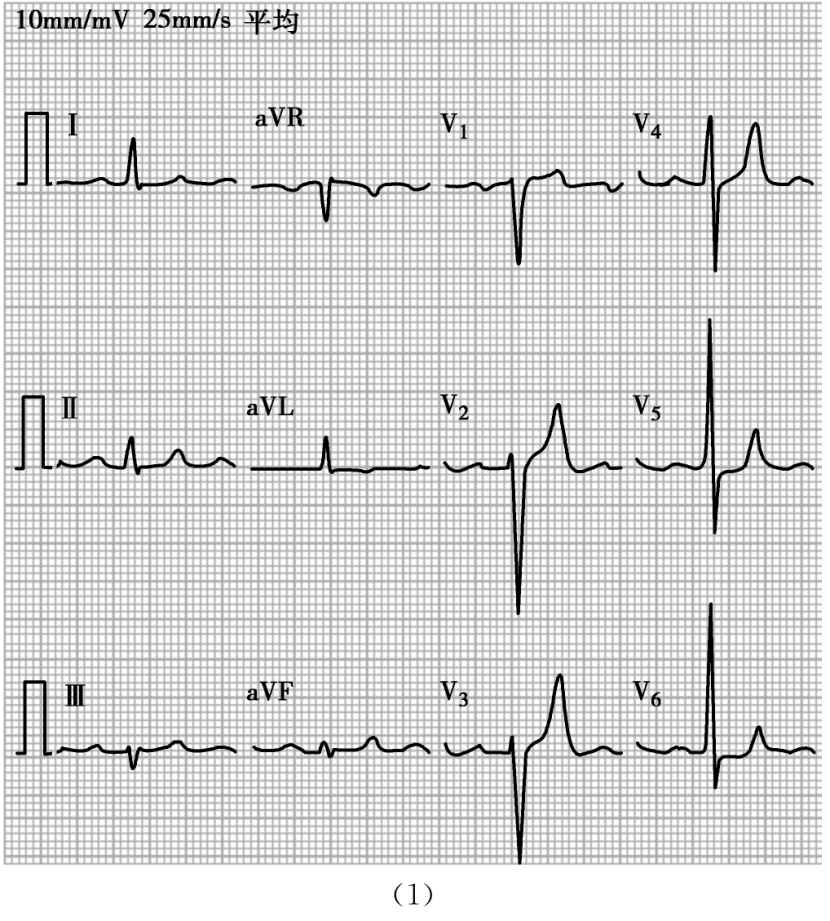
\includegraphics[width=3.38542in,height=3.75in]{./images/Image00070.jpg}

\begin{figure}[!htbp]
 \centering
 
\includegraphics[width=3.19792in,height=3.55208in]{./images/Image00071.jpg}
 \captionsetup{justification=centering}
 \caption{非ST段抬高型心肌梗死心电图}
 \label{fig10-1}
  \end{figure} 

(1)发作前心电图;(2)发生非ST段抬高型心肌梗死时心电图

B.心肌梗死的心电图定位:心肌梗死的心电图定位见表\ref{tab10-2}。

\begin{table}[htbp]
\centering
\caption{心肌梗死定位表}
\label{tab10-2}
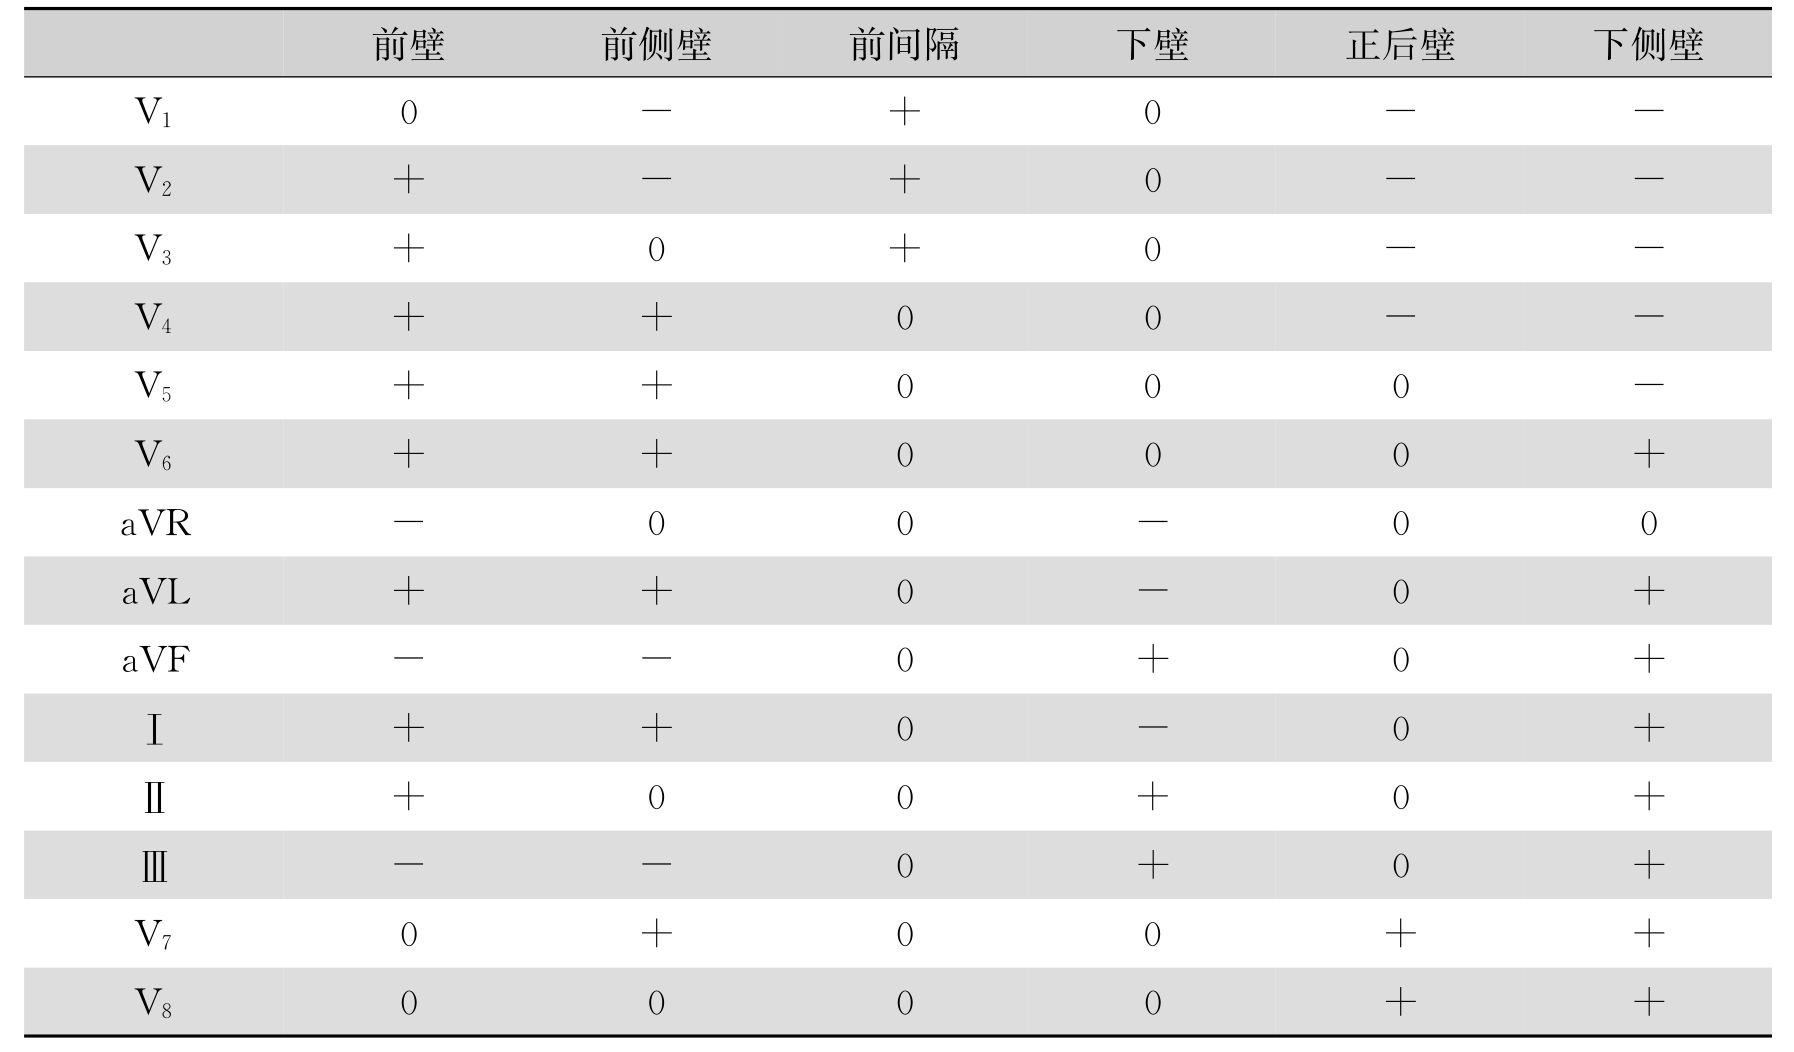
\includegraphics[width=5.96875in,height=3.5in]{./images/Image00072.jpg}
\end{table}

注:“+”指有异常Q波、S-T段抬高及T波倒置的梗死图形;

“-”指与上述相反的变化,如R波增高、ST段压低、T波正向;

“0”无变化

a.急性前壁心肌梗死:急性前壁心肌梗死的特征性图形主要见于胸导联,其次是aVL,临床上常见为前侧壁心肌梗死心电图形(图\ref{fig10-2})。

\begin{figure}[!htbp]
 \centering
 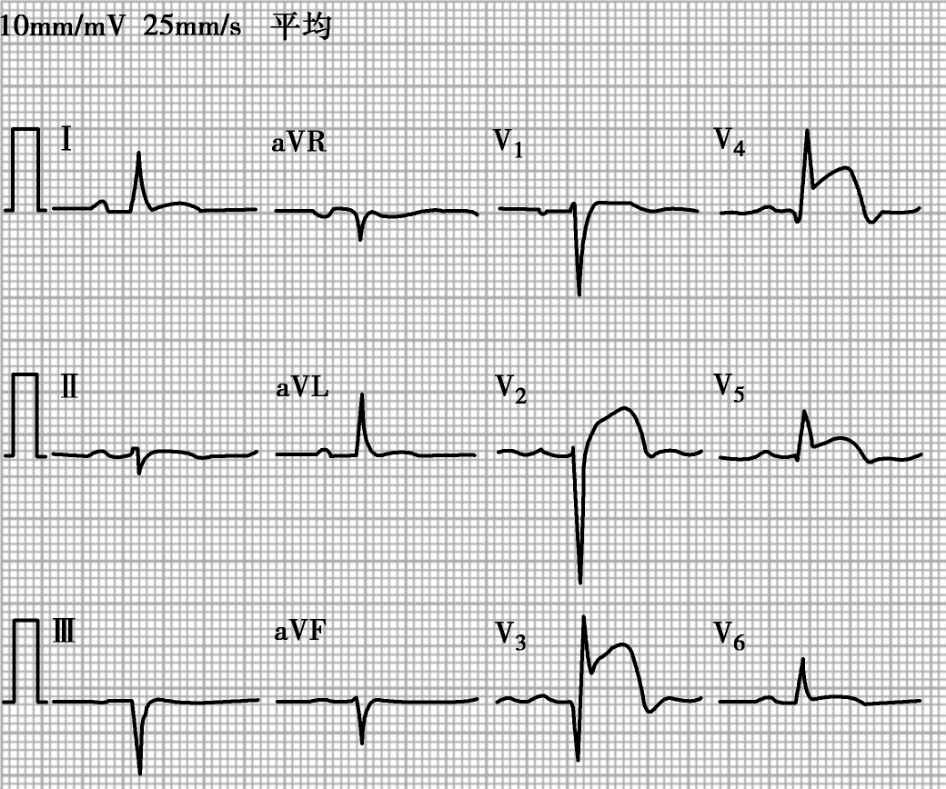
\includegraphics[width=3.45833in,height=2.88542in]{./images/Image00073.jpg}
 \captionsetup{justification=centering}
 \caption{急性前侧壁心肌梗死心电图}
 \label{fig10-2}
  \end{figure} 

b.急性膈面(下壁)心肌梗死:急性膈面(下壁)心肌梗死的特征性图形见于Ⅱ、Ⅲ、aVF;在Ⅰ、aVL及胸导联呈现S-T段下降(图\ref{fig10-3})。

\begin{figure}[!htbp]
 \centering
 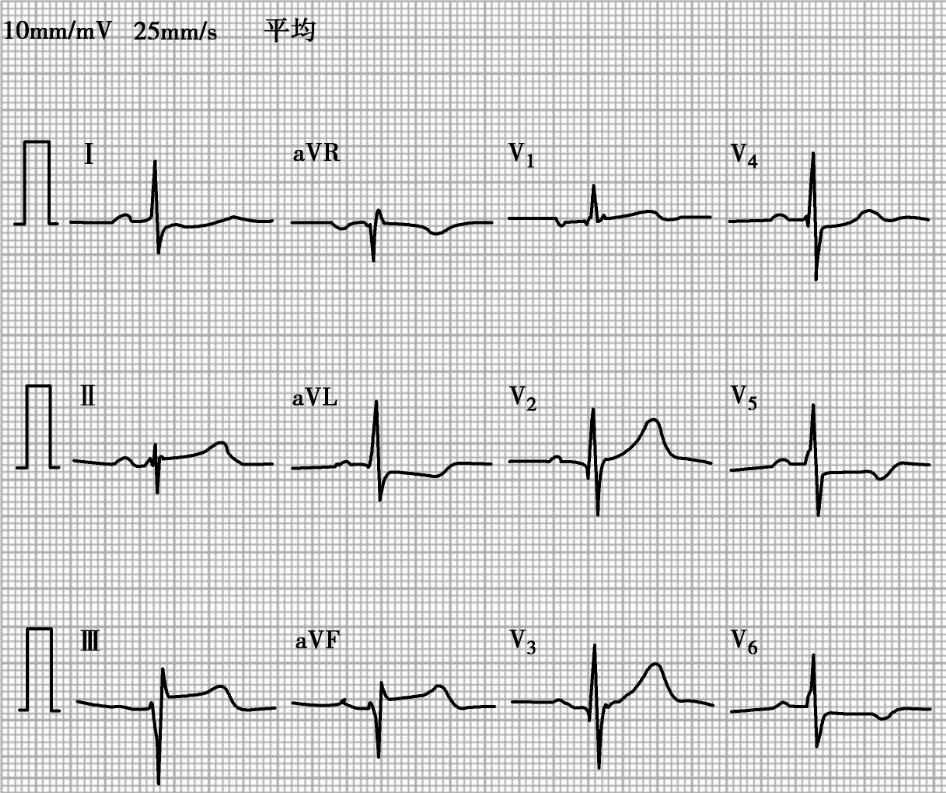
\includegraphics[width=4.05208in,height=3.39583in]{./images/Image00074.jpg}
 \captionsetup{justification=centering}
 \caption{急性下壁心肌梗死心电图}
 \label{fig10-3}
  \end{figure} 

c.急性正后壁心肌梗死:急性正后壁心肌梗死的特征图形见于V\textsubscript{7}
、V\textsubscript{8} ;V\textsubscript{1}
心室波呈RS型或Rs型,R\textsubscript{v1}
顶峰延迟到0.04秒,右胸导联(V\textsubscript{1} 、V\textsubscript{3R}
)S-T段下降,T波直立(图\ref{fig10-4})。下壁心肌梗死常常合并正后壁心肌梗死,因此在Ⅱ、Ⅲ、aVF导联出现下壁心肌梗死的特征性图形时,应特别注意V\textsubscript{7}
、V\textsubscript{8} 导联,以防漏诊正后壁心肌梗死。

\begin{figure}[!htbp]
 \centering
 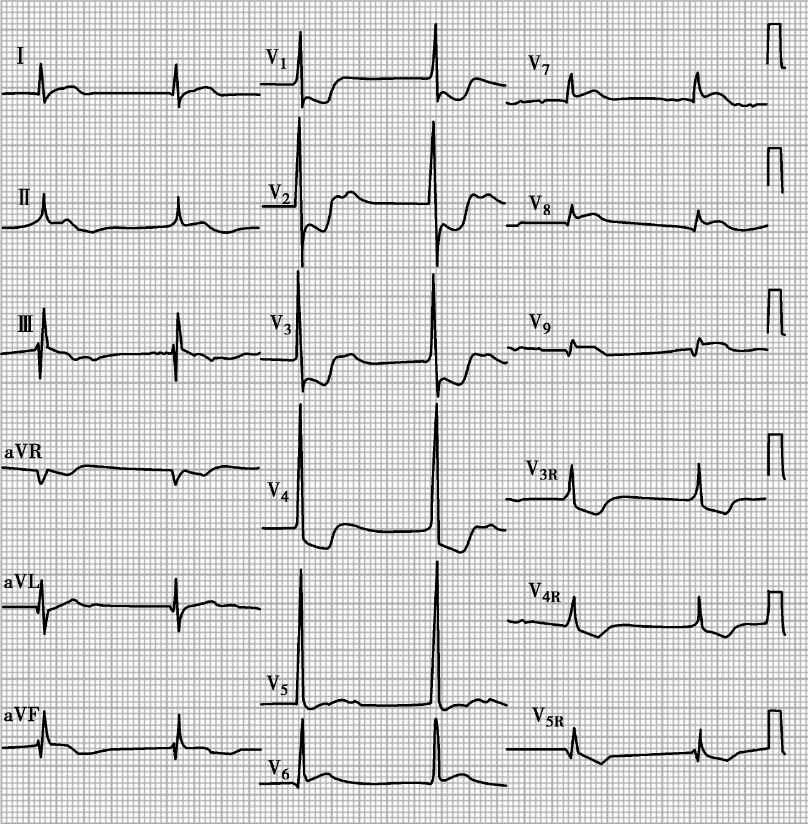
\includegraphics[width=4.33333in,height=4.41667in]{./images/Image00075.jpg}
 \captionsetup{justification=centering}
 \caption{急性下壁合并正后壁心肌梗死心电图}
 \label{fig10-4}
  \end{figure} 

2)关于心肌梗死的漏诊与误诊问题:心电图对心肌梗死的诊断无疑有很大的帮助,然而部分心肌梗死患者的心电图改变是不典型的。相反,一些没有心肌梗死的患者,由于某种原因的影响,可以出现酷似心肌梗死的心电图征象。此外,有些心律失常也可以将心肌梗死图形掩盖。因此,必须结合临床表现及其他实验室检查结果全面考虑,才能提高心肌梗死诊断的准确性,降低假阳性率及假阴性率。现将心肌梗死心电图方面的漏诊与误诊问题讨论如下:

A.有典型的急性心肌梗死临床表现,但心肌梗死图形不典型或心电图无特征性改变时,应作如下考虑:①仅有T波改变的急性心肌梗死。个别患者临床上有典型的急性心肌梗死表现,但心电图仅有T波倒置,倒置的T波在数周内由浅变深,以后又由深变浅逐渐恢复至正常。由于影响T波倒置的因素很多,因此必须符合下列各项条件,才能作出心肌梗死的诊断:临床表现典型,如持续的心前区剧痛、血压下降等;实验室检查,如心肌肌钙蛋白升高,CK,CK-MB升高等;倒置的T波是呈尖锐对称倒置的“冠状T波”,同时其演变过程符合一般心肌梗死的演变规律者。②急性心肌梗死合并完全性左束支传导阻滞时,后者常将前者图形掩盖或使之不典型。③偶见个别急性心肌梗死(尤其室间隔梗死)患者,其急性心肌梗死图形只在室性期前收缩时出现。对这些患者应密切结合临床表现,并定期复查心电图以确定诊断。④一些患者由于心肌梗死部位较特殊,常用的导联及探查部位有时探查不出心肌梗死的图形。疑有此情况时,应增加一些探查部位以提高诊断率。例如:疑为前高侧壁心肌梗死时加做高1
至2肋间部位的左侧胸导联;疑为局限性后壁心肌梗死时加做V\textsubscript{7}
、V\textsubscript{8} 、V\textsubscript{9}
等。⑤急性心肌梗死刚发生不久,心电图可能尚未显示,以后在24小时内,个别在2~3天或更长的时间,复查心电图,心肌梗死图形一般都可出现。

B.急性心肌梗死合并下列的心律失常时,后者常将前者图形掩盖:①阵发性室性心动过速;②室性心律;③完全性左束支传导阻滞;④完全性房室传导阻滞,心室起搏点在房室束以下;⑤预激综合征。

这些患者在心律失常发作前后对比其心电图变化,对诊断有无合并急性心肌梗死有重要意义。

C.在下列情况时心电图可能出现酷似心肌梗死图形而引起误诊:①正常人Q\textsubscript{Ⅲ}
可以超过R\textsubscript{Ⅲ}
的1/4,aVL及aVF也可以出现深的Q波,V\textsubscript{1}
、V\textsubscript{2}
可出现QS波。因此单凭个别深的Q波或QS波来诊断心肌梗死时往往容易误诊,在诊断陈旧性心肌梗死时,更应慎重。②由于风湿性心瓣膜病或梅毒性心脏病等引起的心室肥厚,有时可以出现酷似前壁心肌梗死的图形。③急性肺源性心脏病(急性肺栓塞)时,心电图可出现Q\textsubscript{Ⅲ}
加深,T\textsubscript{Ⅲ}
倒置,应与膈面心肌梗死鉴别。慢性肺源性心脏病心力衰竭严重时,有时也可出现酷似心肌梗死的图形。④束支传导阻滞及预激综合征有时出现的深Q波及ST-T波变化,可酷似心肌梗死的图形。⑤其他如严重的心肌疾病(例如主动脉瓣下狭窄、心脏淀粉样变性、Friedreich遗传性共济运动失调等)、脑血管病,甚至胸前探查电极的移位及呼吸的改变,偶尔也可出现酷似急性心肌梗死的图形。

上述情况有时虽与心肌梗死难以鉴别,但如结合临床表现及有关的实验室检查和及时复查心电图(以上的第②、③、④项情况,如在2天内复查心电图,酷似心肌梗死的图形已消失或变为不典型,则不符合急性心肌梗死心电图的演变过程),全面考虑,综合分析,多能作出正确的诊断。

心肌梗死的确诊需要综合分析临床表现、特征性的心电图改变以及实验室检查发现。细致的多方面检查和动态观察是减少漏诊或误诊的关键。虽然如此,国内仍有报告,临床与病理对照,急性心肌梗死的正确诊断率仅为53\%,而陈旧性心肌梗死为50\%。作者提到急性心肌梗死未能诊断的原因主要是由于并发或伴发于其他疾病、再次梗死、心内膜下心肌梗死或病灶过小。急性心肌梗死临床表现多样化,即所谓“同病异症”,也可能是误诊的一个原因。

急性心肌梗死与心绞痛的鉴别见表\ref{tab10-3}。

\begin{longtable}{c}
 \caption{急性心肌梗死与心绞痛的鉴别要点}
 \label{tab10-3}
 \endfirsthead
 \caption[]{急性心肌梗死与心绞痛的鉴别要点}
 \endhead
 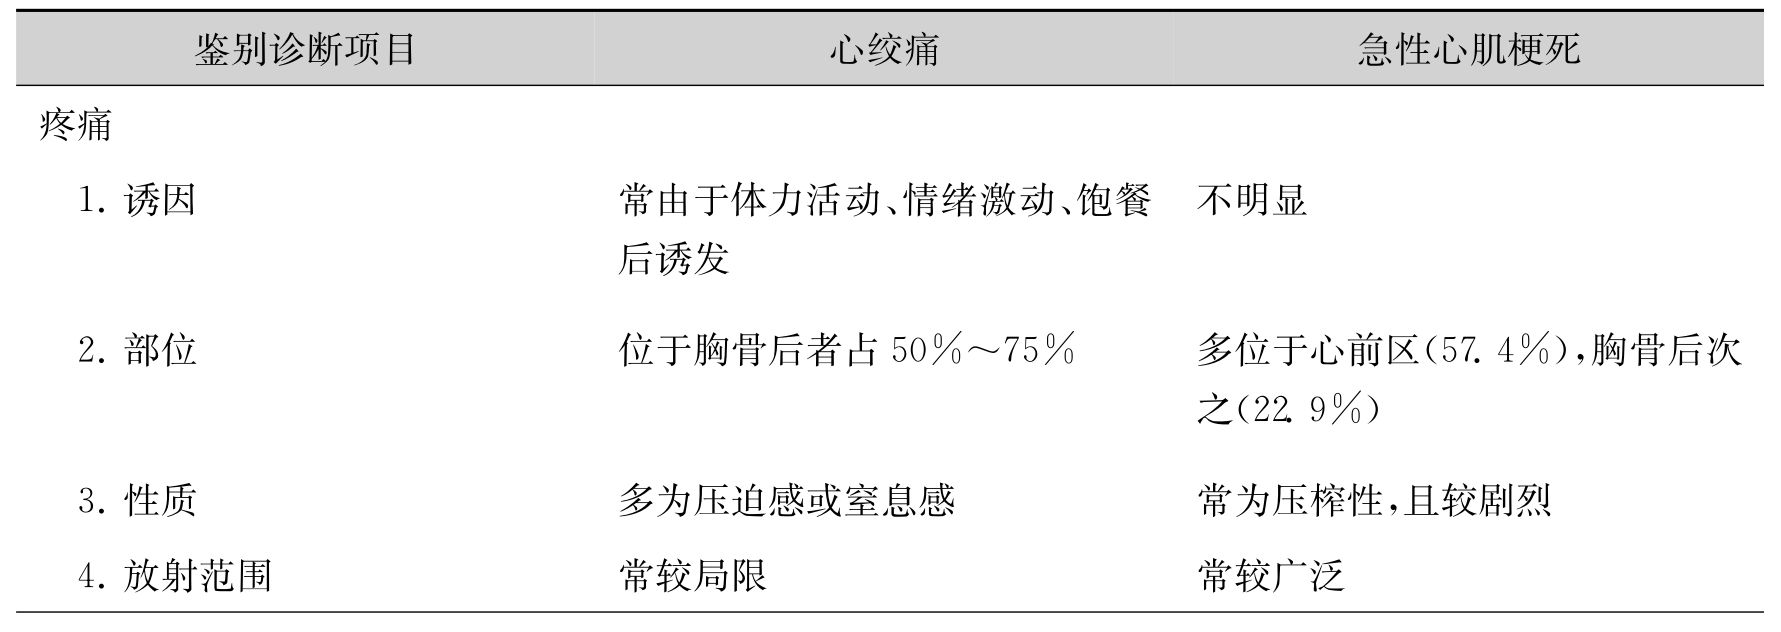
\includegraphics[width=\textwidth,height=\textheight,keepaspectratio]{./images/Image00076.jpg}\\
 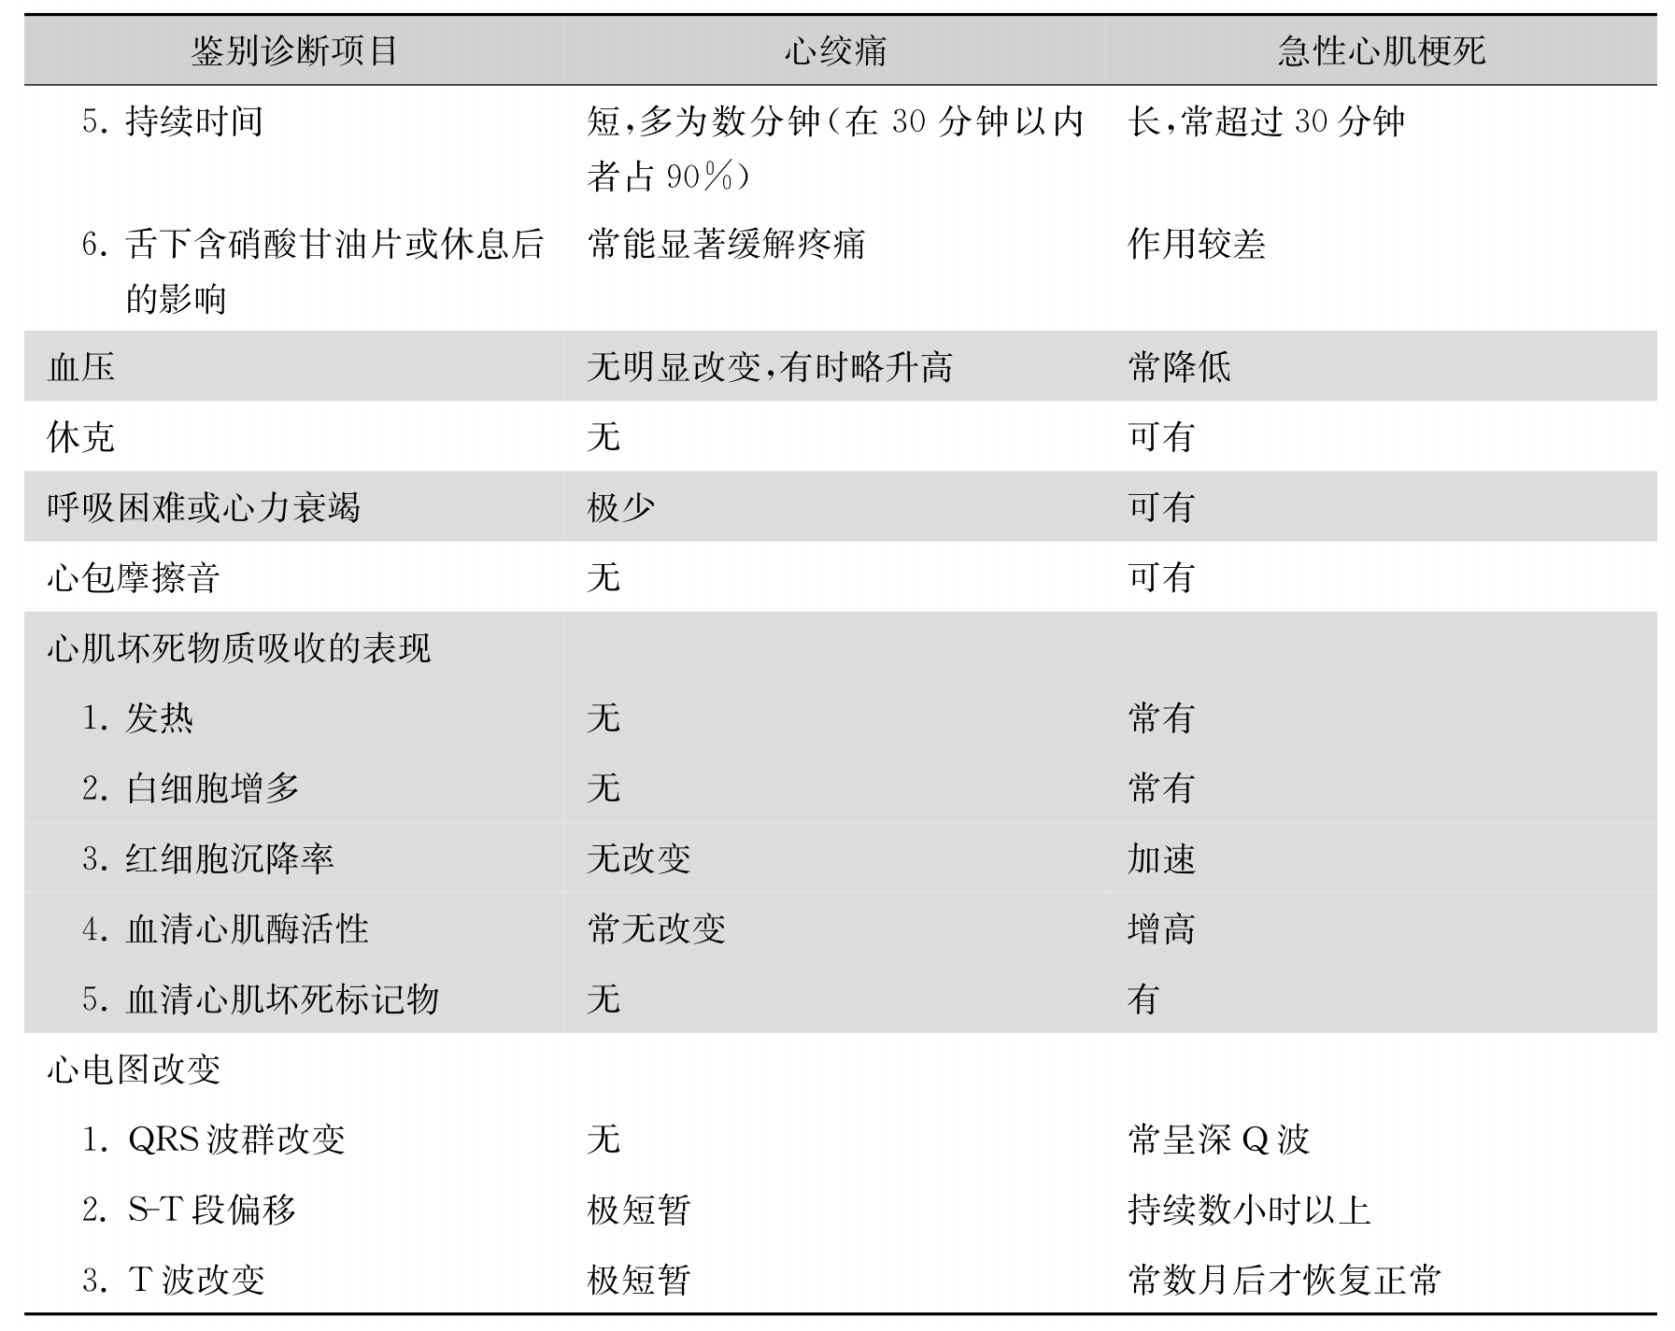
\includegraphics[width=\textwidth,height=\textheight,keepaspectratio]{./images/Image00077.jpg}
 \end{longtable}

急性心肌梗死与急性非特异性心包炎的鉴别见表\ref{tab10-4}。急性心肌梗死尚需与夹层主动脉瘤、肺栓塞相鉴别。

\begin{table}[htbp]
\centering
\caption{急性心肌梗死与急性非特异性心包炎的鉴别}
\label{tab10-4}
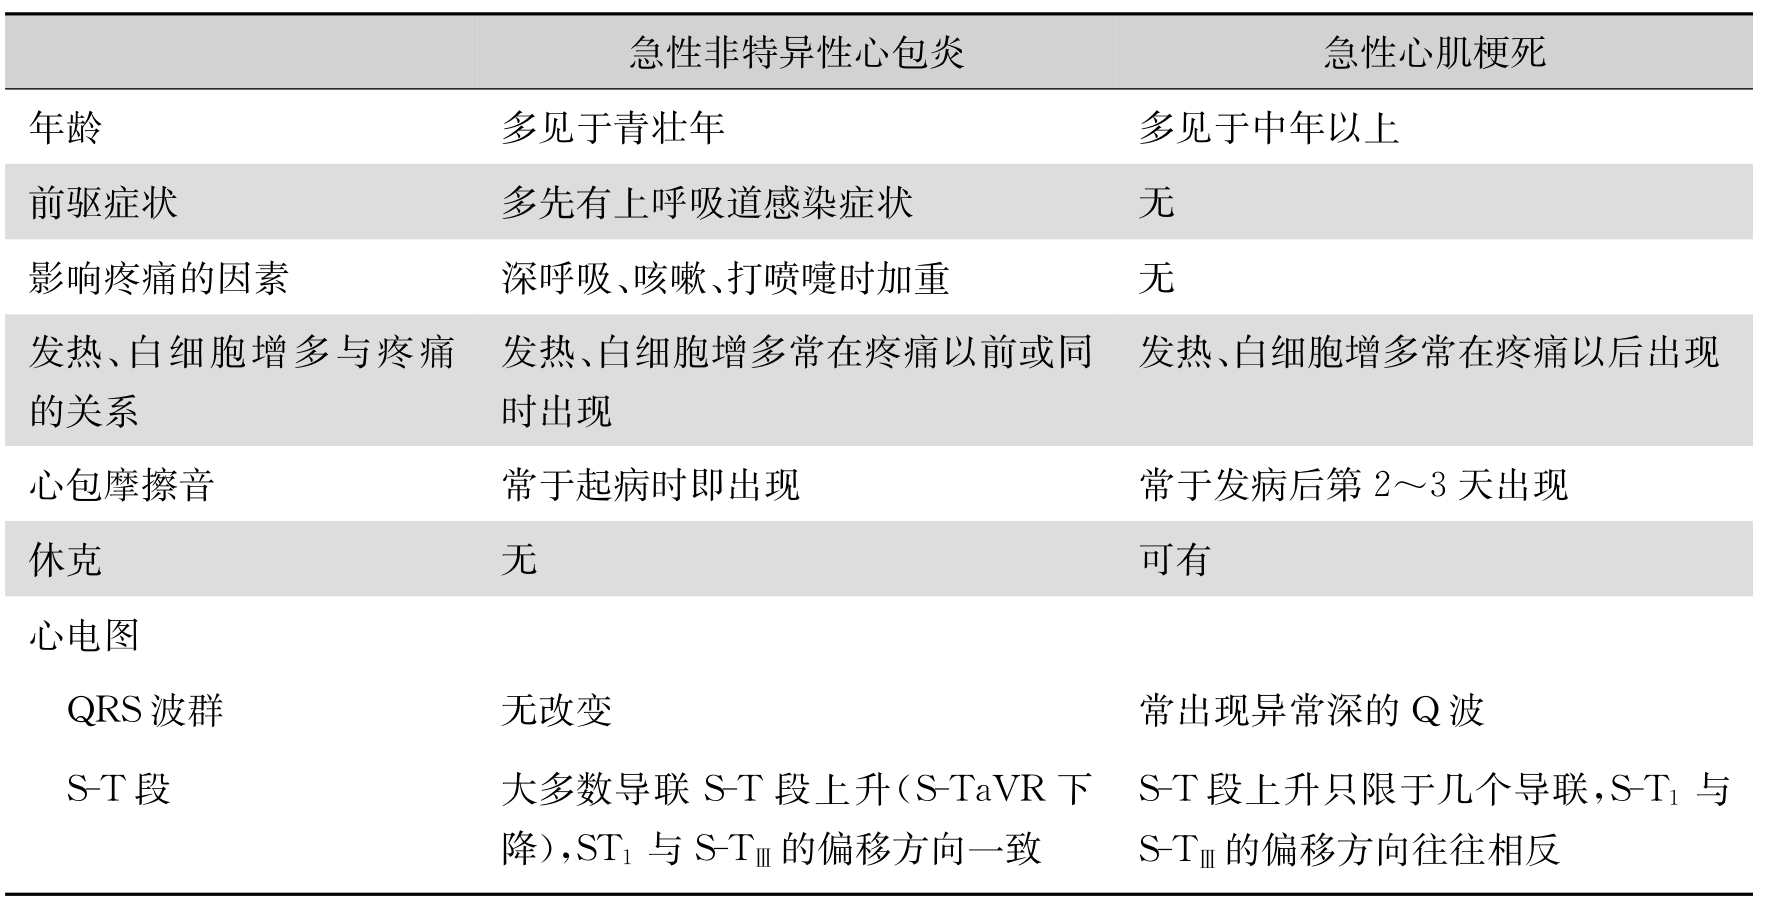
\includegraphics[width=5.91667in,height=3.02083in]{./images/Image00078.jpg}
\end{table}

\subparagraph{(13)冠状动脉造影与心肌显像检查:}

近年国内报道一组47例冠心病,做冠脉造影(CAG)与心肌断层显像(ECT),并比较二者的诊断价值。结果CAG阳性39例,敏感性83\%,特异性100\%,故阳性者诊为冠心病无疑。ECT诊断冠心病敏感性97.9\%(46/47),但特异性仅为45.5\%,因而阳性意义须结合临床,但阴性诊断价值达83.3\%,故阴性者排除冠心病可靠性较大。

有作者进行冠脉造影和\textsuperscript{99m}
Tc-MIBI静息心肌显像(MB)的对比研究。MB是一种安全、无创的检查方法,不仅可直接反映局部心肌血流灌注,也反映冠脉的狭窄程度和范围。结论认为由于冠脉造影与MB有良好的相关性,故MB可作为冠脉造影筛选指标之一,对一些不适宜做冠脉造影的高危患者,MB是一项较好的选择。

有作者分别应用多巴酚丁胺或双嘧达莫(潘生丁)负荷试验下作MB检查,结果提示此法对检测冠脉病变有较高的灵敏性和特异性,且安全,具有较好的诊断价值。

冠状动脉造影的主要指征为:①对药物治疗的心绞痛较严重者,明确冠状动脉病变情况以考虑介入性治疗或旁路移植手术;②胸痛表现似心绞痛而不能确诊者;③中老年患者心脏增大、心力衰竭、心律失常,疑有冠心病而无创性检查未能确诊者。

\paragraph{3.X综合征}

临床上少见,是一种原因不明的发作性心肌缺血。临床表现为劳力型心绞痛。多见于中年女性。发作有明显的诱因,如体力劳动、过度的脑力活动。发作时心电图ST段呈缺血性水平型及下斜型压低。症状缓解后心电图恢复正常,发作时含服硝酸甘油片可缓解。冠状动脉造影正常,有作者认为X综合征的心肌缺血发作与交感神经活性增强有关。

国外作者报道X综合征可能存在微血管功能异常。国内作者检测14例确诊的X综合征患者的血浆内皮素(ET)水平,结果显示X综合征患者血浆ET水平明显高于健康人,而与冠心病患者比较差异无显著性,提示X综合征ET水平升高,可能与心肌缺血及交感神经异常活动有关。内皮素由血管内皮细胞合成释放,是已知体内最强、持续最久的缩血管活性多肽。也有研究报道认为X综合征的病因是由于小冠状动脉扩张储备功能降低或异常收缩而引起的心肌缺血所致。

由于胸痛的原因很多,对冠脉造影正常而有心绞痛样胸痛表现的患者,应根据现有的经验和认识,把那些检出有心肌缺血或冠脉储备功能降低的患者,诊断为X综合征。但有作者还提出,在考虑X综合征诊断时,应该用麦角新碱试验排除心外膜冠状动脉痉挛所致的胸痛;若仍未能诱发冠状动脉痉挛,还需做进一步检查,以评估冠状动脉储备有无异常。此外,还可用核素运动心肌显像或潘生丁负荷试验,诱发胸痛和心电图改变,以判明有无心肌缺血表现。如上述检查均未见异常,则应考虑非心源性胸痛的病因的可能,做相应的检查予以鉴别。

\paragraph{4.心肌梗死后综合征}

发生率约10\%,其发病机制被认为可能系机体对坏死物质的过敏反应。病情经过良好。典型病例其症状发生于急性心肌梗死之后数周到数月内,可反复发生。主要临床表现有持续发热、胸痛、血沉加快、白细胞增多,或并发心包炎、胸膜炎与肺炎。部分病例听诊可闻心包摩擦音,偶尔并发左侧胸腔积液。

肺栓塞后综合征症状与心肌梗死后综合征相似,前者的主要临床特点为:①有肺栓塞的基础疾病;②患者有突然胸痛、气急等症状;③在肺栓塞经过一段时间(一般为3~4周)出现类似心肌梗死后综合征的症状;④短时间的糖皮质激素治疗效果较好;⑤有复发的倾向。

\paragraph{5.冠状动脉瘤}

冠状动脉瘤临床罕见,主要发生于男性,可为单发性或多发性,梭形或囊状。无临床症状时此瘤常不引起注意,但并发血栓形成可发生胸痛,成年患者的胸痛表现与心绞痛相似。疼痛常反复发作数年,在发生心肌梗死后而停止发作。如该动脉瘤穿破至右心(冠状动脉瘘形成),可出现如动脉导管未闭的车轮样连续性杂音。有人认为在无症状的婴幼儿,如胸部X线透视发现房室沟有一非同步搏动的肿块时,提示本病的诊断。冠状动脉瘤常并发于结节性多动脉炎,但也可为先天性、外伤性、真菌栓塞性、梅毒性、动脉粥样硬化性、风湿性等多种病因。有报道腹主动脉瘤常合并动脉粥样硬化性冠状动脉瘤。冠状动脉造影有助于确诊。

据国内有一组冠状动脉瘤12例报告,均在冠状动脉造影中发现,男11例,女1例,6例合并心肌梗死,10例同时合并冠状动脉狭窄(≥75\%),表明本病预后不良。

有一组6例冠状动静脉瘘报告,均为男性。患者以不同程度的胸闷,心悸、体力活动受限等就诊。6例均有心电图持续性ST-T改变,均经冠状动脉造影确诊。由于本病症状、心电图、超声心动图均无特征性,故临床上易于漏诊或误诊。

\paragraph{6.梗阻性肥厚型心肌病(特发性肥厚性主动脉瓣下狭窄)}

本病为常染色体显性遗传病,多在30岁之前出现特征性症状。由于左心室心肌肥厚并累及室间隔,使左心室流出道梗阻,可导致心绞痛发作,并伴有起立或运动后眩晕,甚至神志丧失。超声心动图可显示室间隔非对称性肥厚,舒张期室间隔的厚度与后壁的比例≥1.3。

对临床或心电图表现类似冠心病的患者,如患者较年轻,诊断冠心病依据不充分又不能用其他心脏病来解释,则应想到本病的可能。结合心电图、超声心动图及心导管检查可作出诊断。如有猝死、心脏增大等的家族史更有助于诊断。

\subsubsection{(二)心瓣膜病}

\paragraph{1.二尖瓣膜病}

二尖瓣狭窄或(及)关闭不全均可引起胸痛,发作一般与情绪激动、体力活动及饱餐等因素无关。二尖瓣狭窄所致疼痛的性质以钝痛较为常见,而很少有类似心绞痛样疼痛。体查心尖部可闻及隆隆样舒张期杂音或(及)收缩期吹风样杂音,彩色超声心动图的检查有助于此类病的诊断。

\paragraph{2.二尖瓣脱垂综合征}

胸痛是常见的症状,常为锐痛、刀割样痛或钝痛,疼痛部位常位于心前区,与心绞痛相似。疼痛发作与劳力和情绪变化无恒定关系,也可在休息时发生,疼痛可持续数分钟或数小时,不经治疗可自行缓解。彩色超声心动图的检查有助于诊断。

\paragraph{3.主动脉瓣膜病}

主动脉瓣狭窄或(及)关闭不全均可引起心绞痛发作,前者的发生率在10\%以上,而后者的发生率则少于5\%。主动脉瓣狭窄所引起的心绞痛一般与典型的心绞痛相似,但其特点是较轻度的体力活动更易诱发,含服硝酸甘油片治疗后可引起晕厥。主动脉瓣关闭不全引起的心绞痛常于睡眠中发作,可持续数10分钟至1小时以上,发作时多有血压升高、窦性心动过速及呼吸加快等表现。含服硝酸甘油片治疗常无效或只能起暂时的缓解作用,数分钟后多有重复发作。

主动脉瓣区可闻及响亮的收缩期杂音或(及)舒张期杂音,彩色超声心动图的检查有助于诊断。

\subsubsection{(三)急性心包炎}

急性心包炎,尤其是急性非特异性心包炎,往往有剧烈的胸痛,少数患者只觉紧压感或闷痛,疼痛部位常在心前区,并可放射至左肩、左臂内侧、左肩胛区、背部、颈部、下颌部以及剑突下。疼痛可呈持续性或间歇性发作,于卧位时加重,坐起或身体前倾时减轻。如本病累及邻近胸膜,则胸廓活动增加时(如咳嗽、深呼吸、举臂等)疼痛加剧。体格检查可闻及心包摩擦音,如产生积液可出现心包积液征(Ewart征)甚至出现心脏压塞。

急性心包炎除有心前区剧痛外,还常伴有发热、白细胞增多、血沉加快等,应与急性心肌梗死鉴别(见表\ref{tab10-4})。特异性的心包炎(病毒性、细菌性、结核性)可依靠原发疾病的相关病变进行鉴别。

\subsubsection{(四)先天性心血管病}

肺动脉瓣狭窄、房间隔缺损、肺动脉瓣狭窄合并房间隔缺损(法洛三联症)、法洛四联症、主动脉瓣狭窄、先天性特发性肺动脉扩张,以及特发性肺动脉高压等先天性心血管病,均可发生胸痛。其胸痛的表现可类似心绞痛(占4.8\%),也可类似胸壁痛。这些伴有胸痛的先天性心血管病常伴有肺动脉高压。心脏听诊、心脏X线检查及彩色超声心动图有助于诊断,必要时可做心血管造影以明确诊断。

\subsubsection{(五)胸主动脉瘤}

\paragraph{1.主动脉瘤}

主动脉瘤多由于梅毒性主动脉炎及动脉粥样硬化引起,多由于外伤、感染(如结核、脓毒血症)、风湿病所致,先天性者少见。

主动脉瘤压迫胸壁、脊椎及神经时,均可引起胸痛(约占半数),如压迫其邻近器官则可产生相应的症状。

胸部X线检查可见局限性边缘清晰的梭状或囊状致密阴影,此阴影在任何投照位置不能与主动脉分开。彩色超声心动图也有助于本病诊断。

\paragraph{2.主动脉窦动脉瘤}

主动脉窦动脉瘤(Valsalva窦动脉瘤)大多为先天性,少数由真菌感染与梅毒所致。男性发病多于女性。约3/4的主动脉窦动脉瘤发生在右冠状动脉窦(Valsalva右前窦)的基部,而向右心室穿破。本病国内已有不少病例报告,笔者所在医院也有多例发现。

虽然少数病例可经X线检查发现,但除主动脉窦动脉瘤已发生穿破外,常难以作出临床诊断。在青春期前穿破者不常见。主动脉窦动脉瘤穿破的三联症是:突然出现的颈静脉搏动、动脉脉搏减弱和连续性杂音。症状与体征在穿破时突然出现。胸痛与呼吸困难常突然发生,并呈进行性加重;心力衰竭发生较晚。此动脉瘤常向右心室穿破,引起三尖瓣关闭不全。连续性杂音是其突出的体征,常伴有震颤。此杂音与动脉导管未闭的杂音相类似,但前者在舒张期较响亮,而后者在收缩末期较明显,杂音通常沿胸骨左缘较易听到。以下几点有助于动脉瘤破裂的诊断:①中年以下的患者胸部突然发生疼痛或压迫窒息感,并伴有呼吸困难;②继胸痛之后出现心悸、气短、头痛、头晕或心力衰竭;③心前区可触及明显而广泛的震颤,近胸骨左缘第三、四肋间可闻及Ⅲ~Ⅳ级以上的收缩期与舒张期粗糙的乐音样杂音,舒张晚期增强;④周围血管征阳性;⑤胸部X线检查显示肺血流量增多,心脏向两侧扩大,并呈二尖瓣型。确诊有赖于选择性心血管造影检查。

\paragraph{3.主动脉夹层动脉瘤}

主动脉夹层动脉瘤发病急骤,其特征为运动后突然出现心前区或胸骨后撕裂痛或剧烈的烧灼痛,放射至头、颈、上肢、背、腰、中下腹部甚至下肢,常伴有呼吸困难等其他症状。患者常有高血压病史。

本病可误诊为急性心肌梗死。主动脉夹层动脉瘤时胸痛的特点是放射范围更为广泛,且在剧烈疼痛时仍能维持较高的血压。如夹层主动脉瘤引起无名动脉或左锁骨下动脉阻塞,可致该侧上肢血压较低,脉搏较弱。

主动脉夹层动脉瘤的诊断依据包括:①中年以上有高血压和动脉粥样硬化的病史;②突然发生心前区、背部、腹部或腰部剧烈疼痛;③疼痛发作时有休克征象,但血压仍较高,即使一度下降,但在24~48小时内又复上升,并且很高;④一侧桡动脉搏动减弱或消失;⑤1/5患者主动脉瓣区可听到舒张期杂音;⑥部分患者可出现心包摩擦音或心包、胸腔积液的征象;⑦胸部X线检查可见主动脉阴影进行性加宽,搏动减弱甚至消失;⑧心电图检查无急性心肌梗死的特征性改变;⑨CT、MRI或主动脉造影可见夹层动脉瘤征。

\subsubsection{(六)肺动脉疾病}

\paragraph{1.肺栓塞与肺梗死}

本病常发生于下肢静脉曲张、心脏病、盆腔手术、骨折、长期卧床、老年肥胖等患者。典型的肺栓塞可突然发病,出现呼吸困难、晕厥、发绀、咯血、休克及胸骨后疼痛等症状,如累及胸膜,则吸气时胸痛加剧;如累及膈肌,疼痛可放射至肩部及颈部。肺栓塞典型的心电图改变有肺性P波,电轴右偏,右束支传导阻滞,S\textsubscript{1}
Q\textsubscript{3} T\textsubscript{3}
等,但发生率很低。X线胸片上典型的征象示肺梗死部位呈楔状致密阴影,底部近胸膜,尖端向肺门,也可表现为圆形或多发性不规则阴影,胸腔积液,同侧膈肌上升等。螺旋CT、放射性核素肺灌注和通气扫描、磁共振显像、肺动脉造影有助于明确诊断。本病早期引起疼痛、呼吸困难和心电图改变,应注意与心肌梗死鉴别。

\paragraph{2.肺动脉高压}

不论原发性(特发性)或继发性肺动脉高压均可引起胸痛。检查可发现P\textsubscript{2}
亢进及分裂,心电图出现肺性P波,X线胸片显示肺动脉段明显突出或其高度≥3mm,右肺下动脉干扩张,其横径≥15mm及残根征;肺动脉圆锥≥7mm等可诊断为肺动脉高压。超声心动图和多普勒超声检查可反映肺动脉高压及其相关的表现。

\paragraph{3.肺动脉瘤}

肺动脉瘤是罕见的疾病。大多数为先天性,获得性肺动脉瘤的病因包括慢性肺源性心脏病、梅毒和白塞病。动脉瘤通常位于肺动脉干或其主分支,囊状多于梭状。大的肺动脉瘤可引起咳嗽和呼吸困难,甚至咯血。发生胸痛者占17\%,其疼痛的程度不一,如动脉瘤突然胀大和破裂,则可发生剧烈的锐痛。体查常于肺动脉瓣区出现收缩期杂音和第二音亢进,由于肺动脉瓣环的扩张也可出现粗而长的舒张期杂音。胸部X线检查常显示肺动脉干局限性凸出,肺血管纹理正常,无明显肺门搏动,有助于诊断,但须与纵隔肿瘤及肺癌相鉴别。胸部CT检查或肺动脉造影可确立诊断。

\subsubsection{(七)心血管神经症}

心血管神经症又称Da
Costa综合征,是以心血管疾病的有关症状为主要表现的临床综合征,属于功能性神经症的一种类型。中青年女性较多见,尤其是更年期的妇女。本病的临床意义在于其较易与真正的心绞痛混淆。

本病与典型心绞痛的鉴别要点为:

1.心前区疼痛持续几秒钟到几小时,为短暂的刺痛或较久的隐痛。患者有时觉气闷或呼吸不畅,喜喘一两口大气,或作叹息样呼吸,但无闷痛或较明显的压榨感。

2.胸痛部位多在乳房下或常有变动。

3.症状多出现在劳累后,而不在劳动或兴奋的当时,作轻度体力活动后常感舒适,有时可耐受较重的劳动而不发生胸痛或胸闷。

4.含服硝酸甘油片常无效,或在10多分钟才“见效”。

5.常伴有心悸、疲乏及其他神经衰弱的症状。

心血管神经症的诊断,主要根据上述的特点,以及心血管系统检查的阴性结果。如患者有心前区疼痛,而疼痛的发作与体力劳动无关,虽在休息时仍然存在,或在体力活动后反而减轻,应考虑本病。心血管神经症需与原发性高动力性综合征鉴别,后者被认为由于交感神经活动度过高所致,体查可闻及收缩期喷射音和收缩期杂音,半数患者心电图可显示左心室肥厚。

\protect\hypertarget{text00095.html}{}{}

\subsection{二、呼吸系统疾病}

呼吸系统疾病所致的胸痛,其共同特点是:①胸痛常因咳嗽或深呼吸而加剧;②胸壁局部无压痛;③多伴有咳嗽、咳痰;④常伴有原发病的症状和体征;⑤胸部体格检查与X线检查常可发现病变。

\subsubsection{(一)胸膜疾病}

\paragraph{1.胸膜炎}

由于各种病因所致的胸膜炎的胸痛,在呼吸时加剧,尤其是深呼吸时更明显。干性(纤维素性)胸膜炎的胸痛呈刺痛或撕裂痛,多位于胸廓下部腋前线与腋中线附近,可触及胸膜摩擦感,闻及胸膜摩擦音。膈胸膜炎可引起下胸部疼痛,常向肩部、心前区或腹部放射,可伴有腹壁紧张及压痛而误诊为腹部疾病。渗出性胸膜炎早期为干性胸膜炎,有深吸气时胸痛,随渗出液的增加,胸痛逐渐消失。

\paragraph{2.胸膜肿瘤}

胸膜的原发性或继发性肿瘤均可引起胸痛,尤其是胸膜间皮瘤,其早期为钝痛、刺痛,晚期侵犯肋间神经时出现难以忍受的剧烈胸痛。

胸膜间皮瘤有如下特点时有助于诊断:①患者有石棉接触史;②年龄一般多在40岁以上;③大约60\%患者有胸腔积液,其中3/4为血性胸腔积液伴有进行性胸痛、呼吸困难、乏力、体重减轻和刺激性咳嗽;④胸腔积液透明质酸含量增高,>250mg/L;⑤X线胸片显示胸膜呈不规则状,波浪状阴影,或结节状影,来自胸膜的孤立性肿块,密度高,边缘光滑,呈分叶状;⑥胸腔积液检查可发现恶性间皮细胞瘤细胞。

胸部CT和MRI可评价胸壁和纵隔的受累情况。胸腔镜直视下的活检,不仅可直接观察病变,且取材准确,标本大,阳性率高,是确诊的最佳手段。如果不具备胸腔镜检查条件,必要时也可考虑开胸胸膜活检。

\paragraph{3.自发性气胸、血气胸}

自发性气胸、血气胸常在突然用力后出现一侧剧烈胸痛,伴有呼吸困难,表现有气胸或胸腔积液的体征。部分患者可只觉轻微胸痛,而无明显的呼吸困难,气胸或胸腔积液的体征不明显,易致漏诊。胸部X线检查有助于本病的诊断。

\subsubsection{(二)气管及支气管疾病}

\paragraph{1.支气管炎}

急性支气管炎时因剧烈咳嗽,常引起胸骨后隐痛或紧迫感。慢性支气管炎引起胸痛者少见。

\paragraph{2.原发性支气管肺癌(肺癌)}

早期患者仅有胸闷不适感,随着病情的发展,肺癌侵犯胸膜、肋骨,压迫脊神经后根时可出现持续性胸痛,夜间尤重。疼痛可放射至头颈部或肩部;如放射痛范围广泛,常提示肺癌已有转移。凡中年以上吸烟患者,出现不明原因的胸痛,伴有刺激性咳嗽或血痰,应考虑本病的可能,X线胸片、胸部CT、痰及胸腔积液检查癌细胞、纤维支气管镜检查等可进一步确诊。

\paragraph{3.肺部疾病}

肺部疾病累及胸膜或胸壁时均可引起胸痛。如各种原因引起的肺炎、肺结核、肺栓塞等。

\protect\hypertarget{text00096.html}{}{}

\subsection{三、食管疾病}

食管疾病如食管炎、食管裂孔疝、弥漫性食管痉挛、食管肿瘤、食管憩室、自发性食管破裂等均可引起胸痛,其共同特点是:①疼痛常位于胸骨后;②疼痛多在吞咽时发作或使之加剧;③常伴有吞咽困难。

\subsubsection{1.食管绞痛}

本病是一种食管运动功能障碍性疾病,常见于20~40岁患者,有夜间发作的倾向,患者常从酣睡中痛醒;疼痛位于胸骨后,而向肩胛间区放射。发病时患者可感觉吞咽流质困难,进食冷冻食物可诱发或加剧疼痛。食管绞痛有时相当严重,需用大剂量麻醉剂才能使其缓解,可被误诊为心绞痛,但其特点是不因劳动而诱发,对硝酸甘油的反应差,较少向颈部、下颌与臂部放射。在发作时作食管吞钡X线检查或食管测压,常可发现食管运动功能失调。

\subsubsection{2.胃食管反流病}

本病可引起心绞痛样胸痛发作。在一组52例心绞痛样胸痛的病因分析中,该病占82.7\%,其他原因为食管括约肌高压症占5.8\%,Nutcracker食管占3.8\%。心肌断层显像(ECT)可帮助确定是否有冠心病的存在,食管运动功能检查可明确有无食管运动功能异常及其与胸痛的关系。

另一组关于食管病变所引起的心绞痛样胸痛14例报告,其中男10例、女4例,平均年龄54岁,冠心病的一系列检查阴性,经食管吞钡X线检查、内窥镜检查、食管测压、食管滴酸试验而作出食管病变的诊断。其中弥漫性食管痉挛5例,反流性食管炎与食管裂孔疝各4例,Barrett食管1例。有作者提出食管病变所致心绞痛样胸痛,须符合以下条件:①排除冠心病;②胸痛发作与胃食管反流或食管运动失调在时间上相符;③胃食管反流及食管运动障碍的程度,足以解释胸痛的发生。如患者经奥美拉唑等抑酸药物常规治疗后胸痛消失,更支持胃食管反流所致胸痛的诊断。

24小时食管pH监测法是诊断胃食管反流所致食管源性胸痛的有效方法,还有助于与心源性胸痛的鉴别。

\subsubsection{3.弥漫性食管痉挛}

本病可发生于任何年龄,但以50岁以上多见,主要症状为胸痛和吞咽困难,前者常为心绞痛样,含服硝酸甘油片可缓解。诊断主要依靠食管测压。

\subsubsection{4.急性食管炎}

机械性和化学性损伤是常见病因,胸痛位于胸骨后,可放射到肩部,伴有吞咽困难和疼痛,内镜检查可明确诊断。

\subsubsection{5.自发性食管破裂}

自发性食管破裂(Boerhaave综合征)是在频繁剧烈的呕吐后,食管下段可发生撕裂,进而破入纵隔或胸膜腔,患者常感剧烈疼痛,可出现一侧胸腔积液或积气、皮下气肿等体征。本病应注意与急性心肌梗死、肺栓塞、主动脉夹层动脉瘤、急性胰腺炎及消化道溃疡鉴别,应及早手术治疗。

\protect\hypertarget{text00097.html}{}{}

\subsection{四、胸腺疾病}

由于胸腺炎症、出血、损伤、肿瘤、囊肿等可导致胸痛,但少见。

\protect\hypertarget{text00098.html}{}{}

\subsection{五、纵隔疾病}

\subsubsection{(一)纵隔炎}

\paragraph{1.急性纵隔炎}

急性纵隔炎临床上少见,主要感染途径是:①由于纵隔或邻近器官外伤而感染,这种情况可见于外伤、开放性骨折、食管损伤(由于内镜检查、食管异物、食管癌穿孔)等;②经由血道或淋巴道感染,如并发于脓毒血症、肺炎、急性支气管炎、胸骨骨髓炎、肺脓肿、心包炎及其他细菌感染的过程中。

急性纵隔炎大多为化脓性,主要症状是寒战、高热、白细胞增高和胸骨后疼痛,呈持续性钝痛或钻痛。疼痛因吞咽和深呼吸而加剧。病变部位大多在上纵隔,故常出现前颈部肿痛与压痛。如炎症继发于食管或气管穿孔,可发生纵隔与颈部皮下气肿,出现呼吸困难。X线检查发现纵隔增宽,或兼有纵隔气肿;如形成脓肿,则多在右侧。下纵隔急性炎症的临床表现可与急性上腹部疾病相混淆,详细的病史与X线检查有助于诊断。

\paragraph{2.慢性纵隔炎}

慢性纵隔炎病程缓慢,病因以化脓性或结核性为多,有时为真菌性或梅毒性,症状较急性炎症为轻。结核性纵隔炎常有潮热、乏力、盗汗、消瘦等结核性中毒症状,以及胸痛、咳嗽、吞咽困难等局部症状。如形成冷脓肿,可向食管或气管穿破。化脓性纵隔炎或结核性纵隔炎在炎症吸收之后,可继发广泛性粘连,瘢痕收缩,而引起纵隔器官压迫症状,较多见有不同程度的上腔静脉阻塞综合征。

\subsubsection{(二)纵隔肿瘤}

不论良性或恶性纵隔肿瘤都可引起压迫症状,如压迫神经、胸椎或肋骨,可出现持续胸部疼痛,且常伴有呼吸困难、咳嗽、声音嘶哑、吞咽困难以及上腔静脉阻塞综合征等。X线检查和CT检查对本病有重要的诊断意义。

\subsubsection{(三)纵隔气肿}

纵隔气肿多并发于自发性气胸,但也可由于外伤等原因引起。空气可由以下的途径进入纵隔:①肺泡破裂,空气沿肺间质至肺门进入纵隔;②气管或支气管穿孔;③颈部开放性创伤或皮下气肿;④腹腔内游离空气(气腹)经腹主动脉或食管周围组织进入纵隔。

纵隔气肿较严重时可引起胸痛,常位于胸骨后,常放射至背、颈、肩及臂等处。严重时可引起呼吸困难、发绀及心动过速。颈部、前胸部甚至面部皮下组织因积气而胀满,可触及皮下“握雪感”,叩诊心浊音界缩小或消失,听诊可闻及嚼骨音(Hamman征)于心脏收缩时出现,但此病征并非纵隔气肿所特有,在左侧气胸有时也可听到。后前位X线胸片显示颈部及上纵隔有条索状透亮带,侧位片显示纵隔内心脏与胸骨之间有多数条索状透亮带,提示纵隔内有空气存在。

\protect\hypertarget{text00099.html}{}{}

\section{34 肩关节及其周围组织疾病}

肩关节及其周围组织疾病,如伴有胸肌疼痛及肩、臂痛时,应注意与心绞痛相鉴别。本病无缺血性心电图改变;含服硝酸甘油片症状无缓解;饱餐和情绪激动等不能诱发疼痛发作,活动肩关节及其周围组织可使疼痛加剧。

\protect\hypertarget{text00100.html}{}{}

\section{35 腹部脏器疾病}

\subsection{一、膈下脓肿}

膈下脓肿除有全身性感染症状外,还可引起下胸前部、侧胸或背部疼痛,以右侧较多见,并可放射至肩部。体查发现局部压痛。由于膈下组织炎症与疼痛,可使膈运动减弱。胸部X线检查可见病侧膈肌升高且固定。腹部B超可见膈下肝上有液性暗区,穿刺可抽出液体。

\subsection{二、肝脓肿}

肝脓肿时除有感染症状外,还可出现右下胸痛,疼痛向肩部放射。检查肝区可见局部水肿,有肝区局限性压痛、叩击痛。腹部B超可发现肝脏内有单发性或多发性液性暗区。腹部CT可发现肝脏的单发性或多发性低密度区。

\subsection{三、肝 癌}

尤其是右叶顶部肝癌可引起右下胸痛,并向右肩部放射。检查肝区有轻度叩击痛,腹部B超可见肝脏的占位性病变,腹部CT检查可发现肝脏低密度不规则的阴影,有助于本病诊断。

\subsection{四、消化性溃疡急性穿孔}

消化性溃疡急性穿孔时可引起剧烈的上腹痛,有时也可伴有下胸部疼痛。

\subsection{五、肝胆道疾病}

肝胆道疾病可引起右下胸痛,也可出现类似心绞痛的发作。有时甚至由于胆道症状不明显或被胸痛症状所掩盖,而误诊为冠状动脉粥样硬化性心脏病。因此,如这些患者的心绞痛经积极治疗后改善不显著,又无明显的心血管疾病病征时,应考虑胆道疾病所致的可能性。另一方面,肝胆道疾病伴有胸痛的患者,也可合并冠状动脉粥样硬化性心脏病,且前者可诱发或加重心绞痛的症状。及时做心电图检查,检查胆囊部有无压痛、白细胞计数、胆囊及肝脏的B超检查有助于两病的鉴别。

\subsection{六、脾梗塞}

较大的脾梗塞除可引起恶心、呕吐、左上腹痛外,还可出现左下胸持续性剧痛,并可向左肩和背部放射。此病最多并发于亚急性细菌性心内膜炎,因此常伴有发热、皮肤黏膜出血点、杵状指(趾)、白细胞增高,尿常规检查有红细胞,超声心动图可发现心内膜附着赘生物。

\subsection{七、脾曲综合征}

结肠脾曲胀气的临床表现称为脾曲综合征。脾曲胀气表现为左下胸与左上腹胀痛、便秘等症状,可被误诊为胸膜炎或冠心病。疼痛程度与胀气程度相一致,排便或清洁灌肠后胀气消失时疼痛也消失,症状可骤发或缓发,持续时间不等,以冬季较为多见,一般与饮食关系不大,但与情绪波动有关,发作时腹部X线检查可发现脾曲有明显积气。

\subsection{八、胃心综合征}

胃心综合征主要表现为左侧胸痛或绞窄感,可向左肩放射,偶尔引起心绞痛样发作,易与心绞痛相混淆。本病特点:①患者年龄通常在40岁以下;②有重度吸纸烟和溃疡病史,戒烟后及溃疡病治愈后症状消失;③情绪激动及体力活动后不诱发胸前区痛发作;④消化功能障碍或消化系统疾病治愈后症状缓解;⑤疼痛发作时无缺血性心电图改变,含服硝酸甘油片不能缓解疼痛。

\subsection{九、膈肌病变}

膈肌病变,如创伤性或自发性膈肌破裂、膈肌恶性肿瘤等均可引起胸痛。膈肌破裂常表现为胸痛、胸闷、呼吸困难及恶心、呕吐等消化道症状。创伤性膈肌破裂是急性胸腹腔外伤中少见但严重的合并症,而非创伤性原因所致者称为自发性膈肌破裂,极为罕见,但误诊率高且易出现严重合并症而危及生命。膈肌破裂或膈肌恶性肿瘤的诊断主要依据胸、腹部CT检查。

\protect\hypertarget{text00101.html}{}{}

\section{36 其他原因}

\subsection{一、过度通气综合征}

各种原因引起的过度通气除有呼吸急促、四肢感觉异常、头晕、视物模糊、喉干、甚至意识障碍及抽搐外,还可出现胸痛。其胸痛的特点为:①胸痛性质呈瞬间出现的心前区或左肋弓缘刀割样剧痛,并常放射至颈、背部;②疼痛持续时间数分钟至数小时;③胸骨部有压迫感;④胸部缩窄性疼痛(constrictive
pain),呼吸时随肋间肌收缩而胸痛加剧。易被误诊为心绞痛,但患者有精神紧张、呼吸急促,而无冠心病证据,血气分析显示血pH升高,PaCO\textsubscript{2}
降低常有助于本病的诊断。

\subsection{二、痛 风}

痛风患者除有关节痛外,还可伴有胸痛,疼痛一般呈刀割样,偶尔也可呈钝痛。患者常肥胖,饮酒和高蛋白高嘌呤饮食后疼痛加剧,关节周围可触及痛风石(tophi),血尿酸增高有助于本病的诊断。

\subsection{三、胸廓出口综合征}

由于异常颈肋、前斜角肌病变等压迫臂丛下组和锁骨下动脉,从而产生第8颈神经和第1肋间神经的损害,可引起患侧上胸部及腋下的针刺样或烧灼样胸痛,向患侧颈部、前臂内侧及手掌放射,举物、背物或提物时疼痛加剧。需与颈椎病、颈胸神经根炎及肩关节周围炎相鉴别。

\protect\hypertarget{text00102.html}{}{}

\section{参考文献}

1.晏沐阳,等.胸痛的诊断.中华全科医师杂志,2003,(2):65

2.吴杰,陆再英.常规心电图描记分析方法标准化的进展.中华心血管病杂志,1995,21(1):9

3.荣烨之,朱向阳,不稳定型心绞痛(综述).中华内科杂志,1994,33(8):551

4.许邦龙,等.不稳定性心绞痛临床与冠状动脉造影分析.中华内科杂志,1996,35(5):310

5.陈步星,等.冠状动脉造影评价女性冠心病心绞痛的诊断问题.中华内科杂志,1996,35(4):239

6.李勋,等.冠状动脉造影和心肌断层显像诊断冠心病的对比研究.中华内科杂志,1992,31(10):611

7.陈步星,等.多巴酚丁胺与潘生丁\textsuperscript{99m}
Tc-MIBI心肌显像诊断冠心病价值的比较.中华心血管疾病杂志,1996,24(5):351

8.何作祥,等.多巴酚丁胺负荷试验\textsuperscript{99m}
Tc-MIBI心肌断层显像的临床应用.中华心血管病杂志,1996,24 (1):16

9.王佩芬,等.冠状动造影和\textsuperscript{99m}
Tc-MIBI静息心肌显像的对比研究.中华心血管病杂志,1998,26(3):234

10.支龙,等.ST-T某些改变在冠心病诊断中的价值.中华心血管病杂志,1997,25(1):58

11.李伟扬.X综合征一例.中华内科杂志,1992,31(2):79

12.张澍,等.X综合征患者血浆内皮素浓度变化及其临床意义.中华心血管病杂志,1998,26(2):141

13.徐义枢.关于X综合征的共识与分歧.中华心血管病杂志,1992,20(5):269

14.高润霖,等.X综合征-附六例报告.中华心血管病杂志,1992,20(5):292

15.郭静萱,等.冠状动脉瘤12例临床报告.中华心血管病杂志,1996,20(1):36

16.越成英,等.食管病变所致的心绞痛样胸痛.中华心血管病杂志,1992,20(2):111

17.王世鑫,食管源性胸痛的诊断与治疗.中华全科医师杂志,2003,(2):70

18.柯美云,等.52例心绞痛样胸痛的诊断和治疗.中华内科杂志,1993,32(5):295

19.刘宁,等.30例肺大泡破裂致自发性气胸.中华结核和呼吸杂志,1995,18(6):356

20.陈愉,等.家族性自发性气胸七例.中华结核和呼吸杂志,1998,21(8):509

21.杜志民,等.冠状动静脉瘘心导管检查的临床意义.中华心血管杂志,1995,23(6):448

22.张惠英,等.肺梗塞后综合征二例.中华结核和呼吸杂志,1995,18(1):28

23.李晖,等.弥漫性食管痉挛10例报告.中华消化杂志,1996,16(2):123

24.任菲菲,等.用24小时食管pH值监测法诊断食管原性胸痛.中华外科杂志,1995,33(2):69

25.徐巧莲,等.食管良性溃疡.中华内科杂志,1993,32(5):324

26.王澄,等.创伤性膈肌破裂47例诊断和治疗分析.中国误诊学杂志,2008,8(3):680-681

27.胡敏,等.自发性膈肌破裂的诊断与治疗.山东医药,2007,47(30):49-50

\protect\hypertarget{text00103.html}{}{}

